% Master thesis template for Ghent University (2018)
%
%
%  !!!!!!!!!!!!!!!!!!!!!!!!!!!!!!!!!!!!!!!!!!!!!!!!!!!!!!!!!!!!
%  !!  MAKE SURE TO SET lualatex OR xelatex AS LATEX ENGINE  !!
%  !!!!!!!!!!!!!!!!!!!!!!!!!!!!!!!!!!!!!!!!!!!!!!!!!!!!!!!!!!!!
%  !! For overleaf:                                          !!
%  !!     1. click gear icon in top right                    !!
%  !!     2. select `lualatex` in "latex engine"             !!
%  !!     3. click "save project settings"                   !!
%  !!                                                        !!
%  !!!!!!!!!!!!!!!!!!!!!!!!!!!!!!!!!!!!!!!!!!!!!!!!!!!!!!!!!!!!
%
%
%  History
%    2014         Doctoral Thesis of Bruno Volckaert
%    2017         Adapted to master thesis by Jerico Moeyersons
%    2018         Cleanup by Merlijn Sebrechts
%
%  Latest version
%    https://github.com/galgalesh/masterproef-template
%
\documentclass[11pt,a4paper,twoside, openany]{book}
\usepackage[a4paper,includeheadfoot,margin=2.50cm]{geometry}

\setlength{\parindent}{0cm}           % indent of the first sentence of a paragraph
\setlength{\parskip}{1em}             % space between paragraphs
\renewcommand{\baselinestretch}{1.2}  % stretch horizontal space between everything

\usepackage{graphicx}
\graphicspath{{images/}}
\usepackage{pdfpages}
\usepackage{enumitem}
\usepackage{float}
\usepackage{caption}
\usepackage{subcaption}
\usepackage[toc,page]{appendix}
\usepackage[section]{placeins}
\makeatletter
\AtBeginDocument{%
	\expandafter\renewcommand\expandafter\subsection\expandafter{%
		\expandafter\@fb@secFB\subsection
	}%
}
\makeatother
\usepackage{svg}
\usepackage{amsmath}
\usepackage{graphicx}
\usepackage{epstopdf}
\epstopdfsetup{update} % only regenerate pdf files when eps file is newer
\usepackage[chapter]{minted}                           % for modern code highlighting
\newenvironment{code}{\captionsetup{type=listing}}{}   % To get multiline code fragments working: https://tex.stackexchange.com/a/53540/72273

\AtBeginEnvironment{minted}{\fontsize{9}{9}\selectfont}

\PassOptionsToPackage{hyphens}{url}
\usepackage{hyperref}
\usepackage{url}
\usepackage{quotchap}              % For the fancy quotes next to the chapter titles
\usepackage{wrapfig}               % Handy package to position images
\usepackage[numbers]{natbib}       % For bibliography; use numeric citations
\bibliographystyle{IEEEtran}
\usepackage[nottoc]{tocbibind}     % Put Bibliography in ToC

%
% Defines \checkmark to draw a checkmark
%
\usepackage{tikz}
\def\checkmark{\tikz\fill[scale=0.4](0,.35) -- (.25,0) -- (1,.7) -- (.25,.15) -- cycle;}

%
% For tables
%
\usepackage{booktabs}
\usepackage{array}
\usepackage{ragged2e}  % for '\RaggedRight' macro (allows hyphenation)
\newcolumntype{L}[1]{>{\raggedright\let\newline\\\arraybackslash\hspace{0pt}}m{#1}}
\newcolumntype{C}[1]{>{\centering\let\newline\\\arraybackslash\hspace{0pt}}m{#1}}
\newcolumntype{R}[1]{>{\raggedleft\let\newline\\\arraybackslash\hspace{0pt}}m{#1}}


%
% Own packages added
%
\usepackage[colorinlistoftodos]{todonotes}
\usepackage{xcolor}
\usepackage{tabularx}
\usepackage[acronym,toc]{glossaries} % moeilijke woorden en afkortingen + in toc plaatsen
\usepackage{titling}			   % For \thetitle and \theauthor
\usepackage{multirow} % multi row gebruiken in tables
\usepackage{titlesec, blindtext, color, colortbl}

\usepackage{packages/customcommands}
\usepackage{packages/customcolors}

\renewcommand*{\acronymname}{Lijst van afkortingen}






%
% Support for splitting Dutch words correctly
%
\usepackage{polyglossia}
\setdefaultlanguage[babelshorthands=true]{dutch}

%
% Add support for locally installed fonts and
% add a new command for the UGent font
%
\usepackage{fontspec}
\newfontfamily{\ugentfont}{UGent Panno Text}

% Manually specify additional hypnations for words
\hyphenation{heterogene}

%
% Translated strings. If these aren't set, the English words are used.
%
\addto\captionsenglish{%
  \renewcommand{\contentsname}%
    {Inhoudsopgave}%
}
\renewcommand\appendixtocname{Bijlagen}
\renewcommand\appendixpagename{Bijlagen}
\renewcommand{\listoflistingscaption}{Lijst van listings}
\newfloat{listing}{thp}{lop}
\floatname{listing}{Code}


\newcommand\foreign[1]{\emph{#1}}
\newcommand\inlinecode[1]{\emph{#1}}
%
% Set the title and your name
%
\title{Client-side evaluatie van GeoSPARQL opvragingen over heterogene gegevensbronnen}
\author{Andreas De Witte}
\include{special_chapters/woordenlijst} % lijst van speciale woorden
%
%  END OF HEADER
%  The actual latex document content starts here.
%
\begin{document}
\begin{titlepage}
% Use the main UGent font
{\ugentfont

  % Center the content vertically on the page
  \vspace*{0.37\textheight}

  % Title and author are shown huge
  \begin{huge}

    \thetitle

    \theauthor

  \end{huge}

  \vspace{3.5cm}

  % Promotoren en begeleiding
  \begin{Large}
    Promotoren: dr. ing. Pieter Colpaert, dr. ir. Ruben Taelman\\
    Begeleiding: Brecht Van de Vyvere, Julian Andres Rojas Melendez

    Masterproef ingediend tot het behalen van de academische graad van Master of Science in de Industriële Wetenschappen: informatica
  \end{Large}

  \vspace{1cm}

  % UGent footer
  \begin{Large}
    \begin{wrapfigure}{r}{0.15\textwidth}
      
\includegraphics[width=0.15\textwidth]{ugent.png}
    \end{wrapfigure}

    Vakgroep Informatietechnologie\\
    Voorzitter: prof. dr. ir. Bart Dhoedt\\
    Faculteit Ingenieurswetenschappen en Architectuur\\
    Academiejaar 2019-2020
  \end{Large}
}
\end{titlepage}
           % Front matter
\newpage\thispagestyle{empty}\mbox{}  % White page
% !TeX spellcheck = nl_NL
\thispagestyle{empty}    % Don't show page number
\begin{center}
\textbf{Dankwoord}

Na zes maanden werken is deze masterproef afgerond. Ik heb hier zeer veel aan gewerkt, maar toch zijn er verschillende personen die mij hier mee geholpen hebben.

Als eerste wil ik mijn promotor Pieter Colpaert bedanken voor de continue begeleiding en feedback. Daarnaast wil ik Pieter ook bedanken voor de motivatie en alle opportuniteiten die hij mij gegeven heeft. 

Graag zou ik ook mijn tweede promotor Ruben Taelman bedanken voor de vele technische uitleg en de gegeven feedback over hoe ik mijn thesis tot een beter einde zou kunnen brengen.

Daarnaast wil ik ook graag Ruben Dedecker bedanken voor de gegeven tips over het schrijven, de gezamelijke debug sessies en de raad over het opzetten van de demonstraties.

Tevens zou ik graag mijn mede studenten Demian Dekoninck en Thomas Aelbrecht bedanken voor de steun bij het maken van deze masterproef. Ook van jullie heb ik zeer veel motivatie gekregen, alsook het oplossen van problemen.

Ook zou ik graag mijn familie en vrienden bedanken om altijd klaar te staan voor mij in deze zware periode. Jullie zorgden nu en dan voor de nodige afleiding en ontspanning na een dag werken. Hierbij gaven jullie mij telkens de nodige aanmoediging om door te gaan.

Tot slot zou ik iedereen willen bedanken die mij geïnspireerd heeft voor het schrijven en iedereen die mijn thesis heeft nagelezen. 

Bedankt iedereen!

Andreas De Witte

\end{center}          % Word of thanks
\newpage\thispagestyle{empty}\mbox{}  % White page
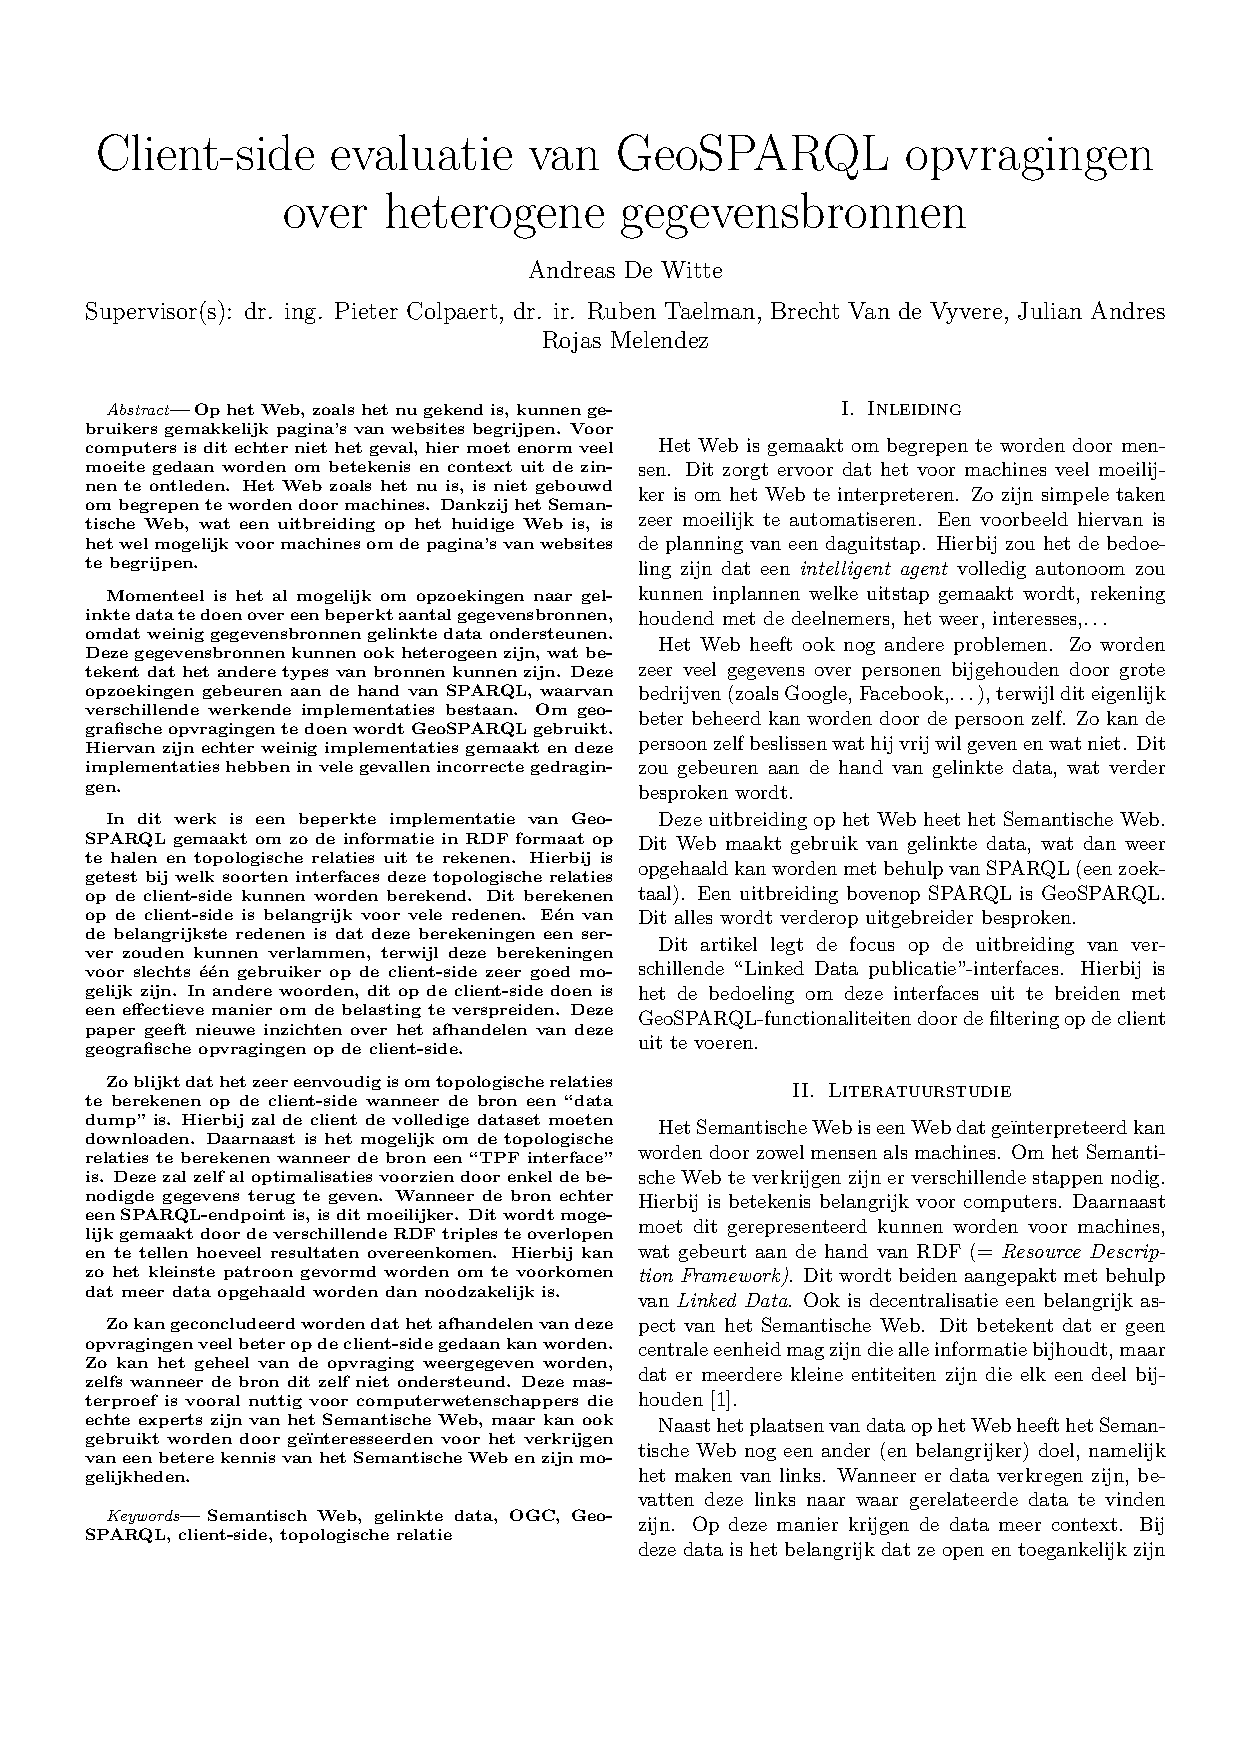
\includepdf[pages={-}]{abstractNL.pdf}  % Extended Abstract not done yet
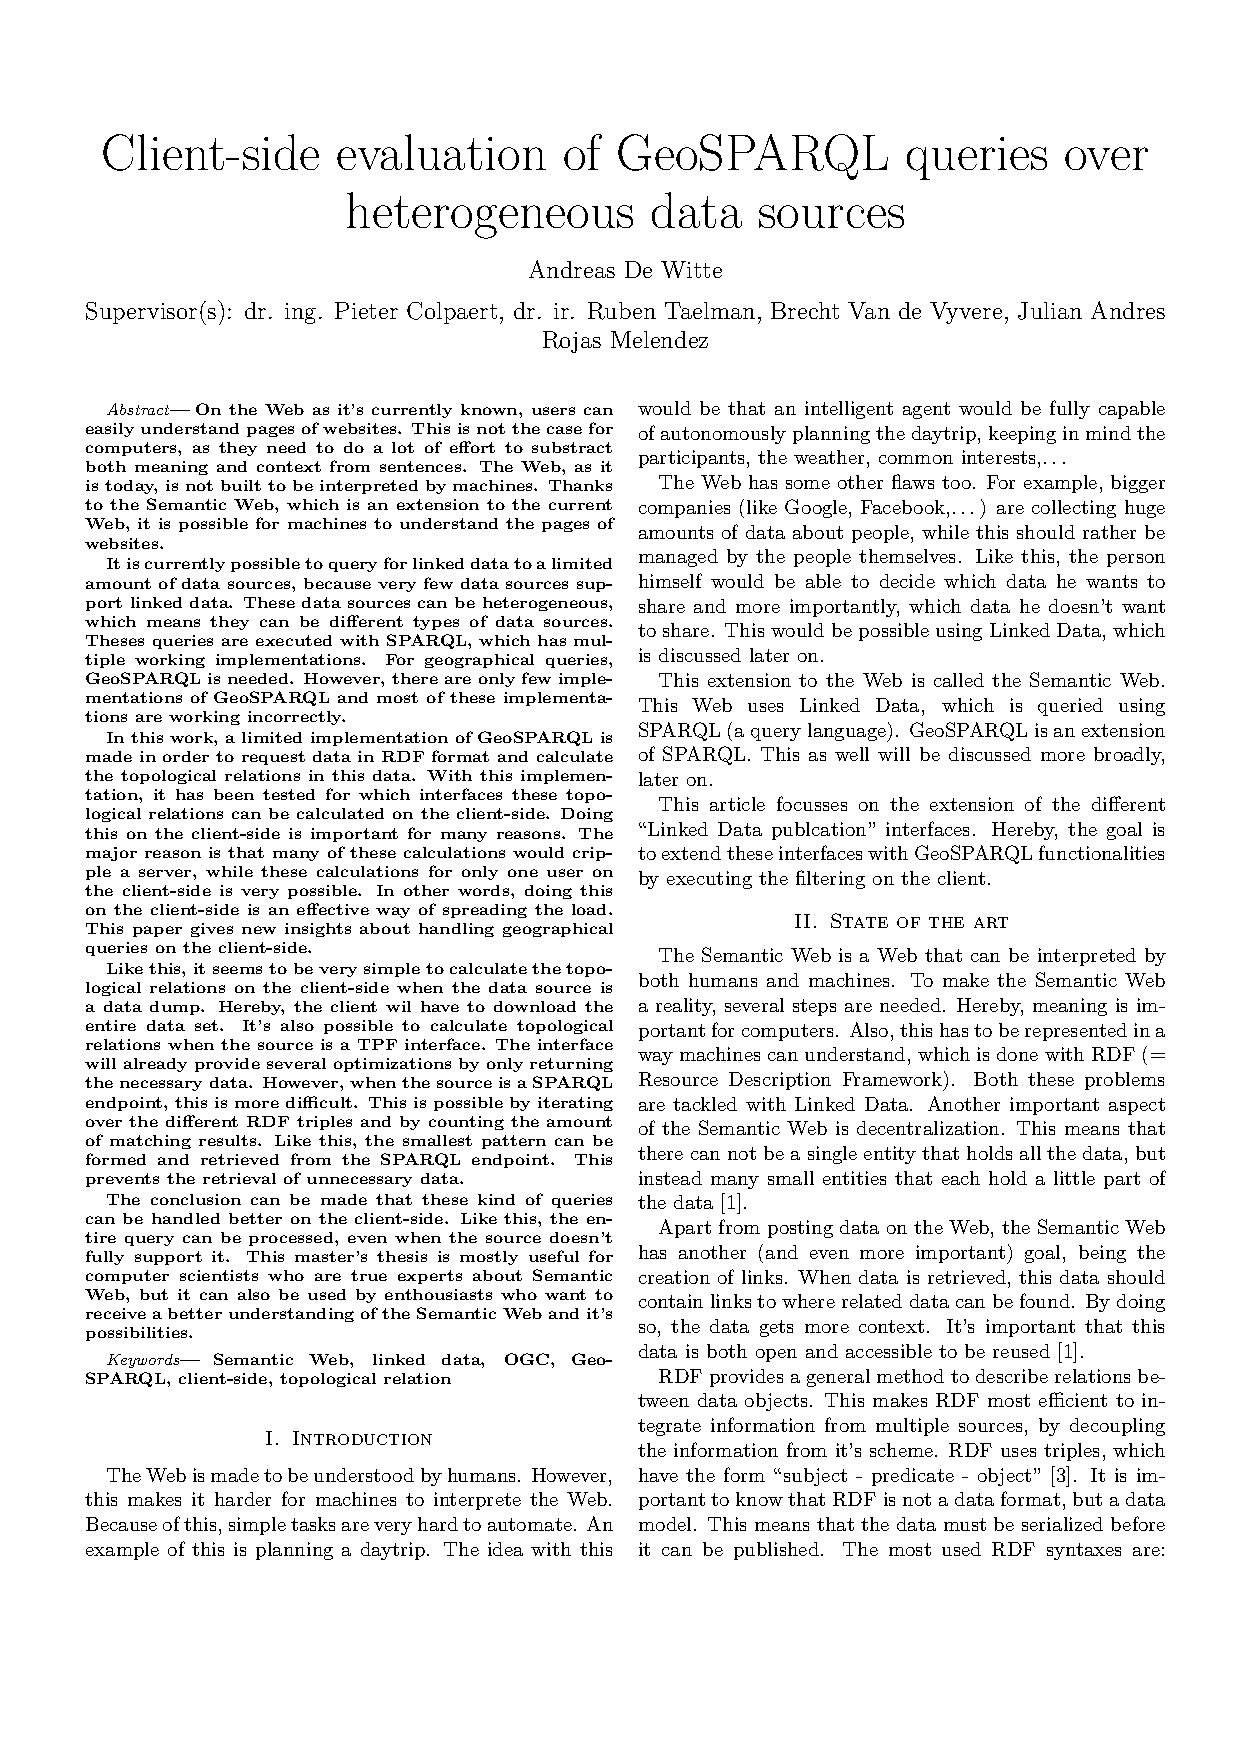
\includepdf[pages={-}]{abstractEN.pdf}  % Extended Abstract not done yet
\tableofcontents                      % Table of Contents


\listoffigures                        % List of figures
\listoftables                         % List of tables
\listoflistings                       % List of listings (code fragments)
\addcontentsline{toc}{chapter}{Lijst van listings} % List of listings in toc
\printglossary % moeilijke woorden tonen
\printglossary[type=\acronymtype] % afkortingen tonen
\todo{lijst van woorden aanvullen en naar verwijzen in tekst!}
\listoftodos 						  % show list of all to do's

% Include the main chapters of the thesis below
%
\chapter{Inleiding}
\chapter{Literatuurstudie}
\section{Semantic Web}
\label{sec:semantic_web}
In 2001 heeft Tim Berners-Lee (uitvinder van het World Wide Web) het over een nieuwe revolutie. Dit is de eerste introductie van het \textit{Semantic Web} (soms wordt er ook naar verwezen onder de term \textit{Web 3.0}). Hierbij zou het web zoals het toen was, evolueren. Zo is het web altijd leesbaar geweest voor mensen, maar niet interpreteerbaar door machines. Het \textit{Semantic Web} zou hier verandering in brengen. Zo zouden machines het web zoals mensen kunnen interpreteren. Deze machines heten \textit{intelligent agents} en zij moeten in staat zijn om complexe taken volledig autonoom uit te kunnen voeren \cite{berners2001semantic}.

Om dit mogelijk te maken zijn er verschillende stappen nodig. Als eerste moet er voor gezorgd worden dat er betekenis gegeven kan worden op een manier die computers kunnen begrijpen. Ook is het belangrijk dat deze kennis gerepresenteerd kan worden aan de machines. Zo wordt er gebruik gemaakt van het RDF model (zie \sectionref{sec:rdf}) met behulp van bijvoorbeeld XML. Verder is het ook belangrijk om er rekening mee te houden dat informatie uit verschillende databanken een andere terminologie gebruikt om hetzelfde uit te drukken. Hiervoor worden verschillende ontologieën gehanteerd (een definitie van de term ontologie wordt gegeven in \subsubsectionref{subsubsec:ontology}). De kracht van het \textit{Semantic Web} zal zichtbaar zijn wanneer er programma's gemaakt worden die informatie kunnen verzamelen van verschillende bronnen (de zogenaamde \textit{intelligent agent}) \cite{berners2001semantic}.

Een belangrijk aspect om het \textit{Semantic Web} mogelijk te maken is dus decentralisatie. Hiermee wordt bedoeld dat de macht (hier in de vorm van informatie) niet in handen mag zijn van enkele grote spelers, maar verspreid moet worden. In een ideale vorm van het \textit{Semantic Web} zou elke persoon een \textit{pod} hebben die de informatie over zichzelf bevat. Wanneer een website toegang tot deze informatie zou willen, dan zou deze informatie uit de \textit{pod} opgehaald moeten worden. Dit zou nog andere voordelen brengen, zoals onder andere een verbeterde privacy (toegang verlenen aan wie de persoon wil).

\subsection{Semantic Web Stack}
De architectuur van het \textit{Semantic Web} gebaseerd is op een hiërarchie van talen, waarbij elke taal de mogelijkheden van de talen lager in deze hiërarchie optimaal zal benutten en uitbreiden. Deze hiërarchie is gevisualiseerd in \figureref{fig:semantic_web_stack}, ontworpen door Tim Berners-Lee. In de paper ``Semantic Web Architecture: Stack or Two Towers?'' worden alternatieve voorstellingen van de \textit{Semantic Web Stack} besproken \cite{horrocks2005semantic}. In deze masterproef wordt niet verder ingegaan op deze uitbreidingen. De lagen van de oorspronkelijke \textit{Semantic Web Stack} die belangrijk zijn voor deze masterproef, worden hieronder besproken.

\begin{figure}[ht]
    \centering
    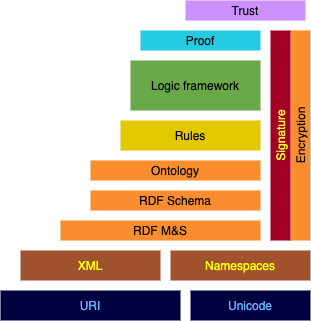
\includegraphics[width=0.5\linewidth]{images/Semantic-Web-Stack.png}
    \caption{Semantic Web Stack (gebaseerd op \textit{Semantic Web Stack} \cite{semanticwebstack})}
    \label{fig:semantic_web_stack}
\end{figure}

De volgende delen zullen de talen die van belang zijn voor deze masterproef bespreken.

\subsubsection{Unicode}
Unicode is een systeem dat gebruikt wordt voor het encoderen van karakters. Net zoals ASCII is het ontwikkeld om ontwikkelaars te ondersteunen bij het maken van applicaties. Unicode pakt de problemen aan van eerdere karakter encodeer systemen, zoals onder meer het niet-ondersteunen van alle karakters. Zo zal unicode een uniek nummer hebben voor elk karakter op elk platform, voor elk programma en in elke taal \cite{unicode}.

Unicode ligt aan de basis van de \textit{Semantic Web Stack} omdat het \textit{Semantic Web} documenten in verschillende talen moet kunnen doorgeven. Deze documenten moeten dus ook kunnen gerepresenteerd worden.

\subsubsection{URI}
URI staat voor \textit{Uniform Resource Identifier}. Dit is een uniforme manier voor het identificeren van objecten. Deze term wordt soms door elkaar gehaald met de term URL, wat staat voor \textit{Uniform Resource Locator}. Het grote verschil tussen beiden is dat een URI een object kan identificeren (= hoe iets te benoemen), terwijl een URL een object kan localiseren (= waar iets te vinden). De verwarring tussen beiden komt door hun onderlinge relatie. Om dit verschil te begrijpen is het belangrijk te weten dat de verzameling van URL's een subset is van alle URI's. Zo is elke URL een URI, maar niet omgekeerd \cite{uri}.

Samen met unicode ligt URI mede aan de basis van de \textit{Semantic Web Stack}. Zowel URI als unicode maken het mogelijk om op het Web resources te identificeren op eenzelfde eenvoudige manier.

\subsubsection{XML}
XML staat voor \textit{Extensible Markup Language}. Het wordt gebruikt voor de beschrijving van data. Eén van de belangrijkste kenmerken van de XML standaard is het vermogen om op een zeer flexibele manier data te structureren. Het W3C \todo{in verklarende woorden plaatsen}beveelt XML dan ook aan. XML werkt aan de hand van elementen die gedefinieerd worden door \textit{tags}. Zo heeft elk element een begin -en een eind\textit{tag}. XML ondersteunt ook geneste elementen zodat echte hiërarchiën gemaakt kunnen worden. XML is dus belangrijk gezien zijn eenvoud en uitbreidbaarheid \cite{bray2000extensible}. 

\subsubsection{Namespaces}
XML Namespaces worden ook aanbevolen door het W3C. De reden hiervoor is om te voorkomen dat verschillende elementen dezelfde en dus conflicterende namen hebben. Op deze manier wordt de woordenschat gedifferencieerd, zodat deze woordenschat herbruikt kan worden. Het idee van namespaces steunt volledig op de werking van URI \cite{bray1999namespaces}.

\subsubsection{RDF Model, Syntax en Schema}
RDF staat voor \textit{Resource Description Framework}. RDF zal op een beschrijvende manier informatie geven. RDF is echter te belangrijk om kort besproken te worden en zal dus uitvoerig besproken worden in \sectionref{sec:rdf}.

\subsubsection{Ontology}
\label{subsubsec:ontology}
Het woord \textit{ontology} zorgt voor veel verwarring en heeft bijgevolg al meerdere verschillende definities gekregen. In zijn artikel ``What is an ontology?'' beschrijft Tom Gruber een ontologie als een specificatie van een conceptualisatie. De term ontologie komt van de filosofie waar het de betekenis heeft van een systematisch teken van het bestaan. Een ontologie kan beschreven worden als het definiëren van een set van representerende termen. Zo zullen relaties tussen objecten beschreven worden in een vorm die begrijpbaar is door mensen. Formeel betekent dit dat een ontologie een uitspraak is van een logische theorie \cite{gruber2018ontology}. 

In de computerwetenschappen refereert de term ontologie naar een formele beschrijving van kennis. Zo kan informatie die van verschillende bronnen komt vertrouwen op de ontologieën om een gelijkaardige betekenis te krijgen.
\newpage
\section{Linked Data}
\label{sec:linked_data}

Het semantisch web gaat echter niet enkel over het plaatsen van data op het web. Het belangrijkste aspect van het semantisch web is het maken van links, zodat zowel personen als machines het web van data kunnen doorkruisen. Het belangrijke van gelinkte data kan als volgt omschreven worden: wanneer je data hebt, kan je er andere gerelateerde data mee vinden. Bij gelinkte data worden deze links beschreven aan de hand van RDF. Hierbij worden URI's gebruikt voor het identificeren van objecten. Om data te interconnecteren zijn er vier regels, met als doel dat de informatie in de toekomst op onvoorspelbare manieren herbruikt zou kunnen worden. Daarnaast is het belangrijk dat de data open en toegankelijk zijn om herbruikt te worden \cite{berners2006linkeddata}. 

\subsection{Regels}
Bij gelinkte data zijn er vier regels waaraan voldaan moet worden:
\begin{enumerate}
    \item Dingen moeten geïdentifeceerd worden met URI's. Dit is nodig om te kunnen spreken over een semantisch web \cite{berners2006linkeddata}. 
    \item Er moet gebruik gemaakt worden van HTTP URI's. Dit is nodig zodat andere gebruikers de namen zouden kunnen opzoeken \cite{berners2006linkeddata}. 
    \item Bijhorende informatie moet gevonden kunnen worden wanneer een URI gevolgd wordt. Dit is in het basis formaat van RDF en XML. Deze kan ook doorzocht worden aan de hand van SPARQL (verder besproken in \sectionref{sec:sparql}), dit is een query service voor gelinkte data in RDF formaat \cite{berners2006linkeddata}. 
    \item Er moeten links voorzien zijn naar andere locaties die gelijkaardige data bevat, zodat dit opgezocht kan worden. Deze laatste regel is belangrijk om de informatie op het web te connecteren \cite{berners2006linkeddata}.
\end{enumerate}

\subsection{Vijfsterrenmodel}
Het vijfsterrenmodel is een manier om informatie in te delen in hoeverre ze open is. Meer sterren betekent dat de informatie meer open is. Tim Berners-Lee stelde dit model voor als schema voor gelinkte open data. Gelinkte open data is een essentiëel onderdeel van het semantisch web.

Eén ster stelt hetvolgende: ``\textit{Available on the web but with an open licence, to be Open Data}''. Dit betekent dat gebruikers informatie kunnen ophalen, gebruiken en delen met iedereen. Het gaat hier echter louter over het delen van informatie, het maakt dus niet uit in welk formaat dit komt \cite{berners2006linkeddata}. 

Twee sterren stelt dan weer: ``\textit{Available as machine-readable structured data}''. Om twee sterren te krijgen is het belangrijk dat de informatie een bepaalde structuur heeft, zodat machines deze informatie kunnen verwerken. Dit kan bijvoorbeeld zijn in de vorm van een excel spreadsheet. Dit soort informatie is echter nog steeds vrij gesloten aangezien de gebruikers afhankelijk zijn van bepaalde software om toegang te krijgen tot de informatie \cite{berners2006linkeddata}.

Drie sterren betekent: ``\textit{The same as 2 stars, plus non-proprietary format}''. Het verschil om van twee sterren naar drie sterren te stijgen is het vermijden van de nood aan specifieke software om de informatie te bemachtigen. Dit kan bijvoorbeeld door de informatie op te slaan in CSV formaat \cite{berners2006linkeddata}.

Vier sterren is vervolgens: ``\textit{All the above plus, use open standards from W3C to identify things, so that people can point at your stuff}''. Voor het verdienen van de vierde ster moet de informatie voldoen aan de open standaarden van W3C. Zo moet het dingen identificeren aan de hand van RDF of SPARQL. Hierbij is het belangrijk dat gebruikers (aan de hand van URI) kunnen verwijzen naar de data \cite{berners2006linkeddata}.

Tenslotte betekent vijf sterren hetvolgende: ``\textit{All the above, plus: Link your data to other people’s data to provide context}''. Om de laatste ster ook te kunnen behalen, dient men de informatie te linken aan bijhorende informatie in een andere context. Op deze manier worden de links verder verspreid. Hier wordt er dus letterlijk verwezen naar andere locaties, met als doel om meer context terug te vinden \cite{berners2006linkeddata}.

\subsection{Linked data gevisualiseerd}

\begin{figure}[ht!]
    \centering
    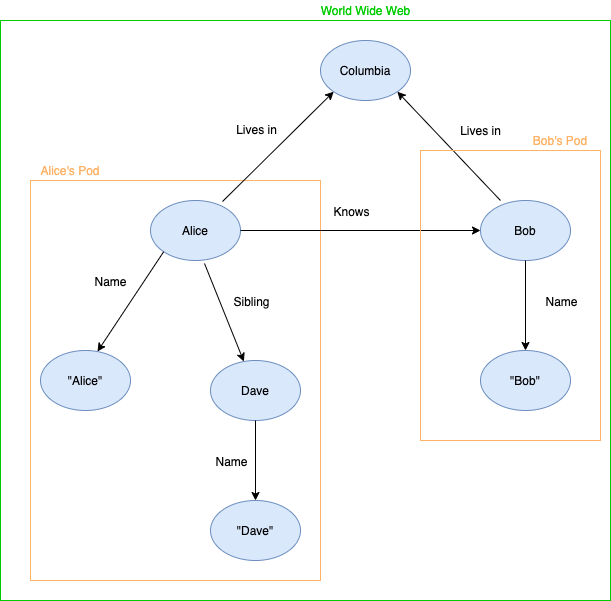
\includegraphics[width=\linewidth]{Linked-Data-Example.png}
    \caption{Linked Data voorbeeld}
    \label{fig:linked_data_example}
\end{figure}

Een voorbeeld van hoe het \textit{World Wide Web} eruit zou kunnen zien is geschetst in \figureref{fig:linked_data_example}. Dit voorbeeld toont de ideale situatie waar personen een eigen pod met informatie hebben. Zo hebben Alice en Bob elk hun eigen plaats in het web, waar informatie over hun te vinden is. Deze informatie zou onder andere hun naam, telefoonnummer, adres, interesses, werkomgeving, etc kunnen zijn. Daarnaast zijn er ook connecties tussen Alice en Bob. Om te beginnen is Bob gekend door Alice, waardoor er een verwijzing is naar meer context over Bob in zijn pod. Daarnaast wonen ze beide in dezelfde stad, waardoor het mogelijk is om bijvoorbeeld te zoeken naar iedereen die in een bepaalde stad woont. Al deze personen zullen terug te vinden zijn aan de hand van een verwijzing naar meer context (lees: meer informatie) gelinkt aan personen. Dit is echter een vereenvoudigd voorbeeld, in de reële situatie zijn er veel meer links en dit in meerdere richtingen.
\newpage
\section{RDF}
\label{sec:rdf}

RDF staat voor \textit{Resource Description Framework}. Het \textit{World Wide Web} is gemaakt voor mensen, en hoewel machines het kunnen lezen kunnen ze het niet altijd interpreteren. Het doel van RDF is om een algemene methode te voorzien om relaties tussen data objecten te beschrijven. Zo is RDF ontstaan in een poging om metadata te maken. Metadata worden gezien als data over data, maar kunnen beter geïnterpreteerd worden als data die \textit{web resources} beschrijven. RDF blijkt een zeer effectieve manier om informatie van verschillende bronnen te kunnen integreren door de informatie los te koppelen van zijn schema. Op deze manier kunnen de gegevens ook tegelijkertijd opgezocht worden. Zo poogt het dus om informatie op het web interpreteerbaar te maken voor machines. RDF steunt op de bestaande web standaarden zoals XML en URI. XML is echter slechts een mogelijke syntax. Er zijn verschillende andere manieren mogelijk om dezelfde RDF data te representeren. Het algemeen doel van RDF is het definiëren van een mechanisme. Dit mechanisme zorgt voor het beschrijven van \textit{resources} die geen veronderstellingen maken van een specifiek domein, noch een semantiek definiëren \cite{lassila1998resource}.

\subsection{RDF data model}
\begin{figure}
    \centering
    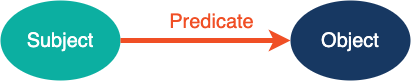
\includegraphics[width=0.5\linewidth]{images/spo.png}
    \caption{RDF statement}
    \label{fig:spo}
\end{figure}

De onderliggende structuur van een RDF uitdrukking is een collectie van triples. Elk van deze triples bestaat uit een \textit{subject} (= onderwerp), \textit{predicate} (= eigenschap) en \textit{object} (= voorwerp). Zoals te zien is in \figureref{fig:spo}, kan dit geïllustreerd worden als een \textit{node-arc-node link} (\textit{node} is een knoop, terwijl \textit{arc} een tak is). Deze collectie van triples kan bijgevolg gezien worden als een graaf. Hierbij is de richting van de \textit{arc} belangrijk, deze wijst in de richting van het \textit{object}. \cite{klyne2009resource}.

Eén enkele triple weerspiegelt een eenvoudige zin. Bij een kort terugblikken naar \figureref{fig:linked_data_example} is hetvolgende triple te zien: (\textit{Alice - Knows - Bob}). Deze triple staat letterlijk voor de zin ``\textit{Alice knows Bob}''. Deze zin hoeft echter niet altijd een exacte vertaling te zijn, bij een ander voorbeeld zien we dat er enkele korte woorden toegevoegd moeten worden om een gramaticaal correcte zin te bekomen: (\textit{Alice - Name - ``Alice''}) wordt dan weer ``Alice has name Alice''. In dit voorbeeld gaat het nu over de naam, maar het kan hier evenwel over een emailadres of een leeftijd gaan.

\subsubsection{URI-gebaseerde vocabulair}
Een \textit{node} kan een URI, een \textit{literal} of \textit{blank} zijn. Een URI referentie of een \textit{literal} die gebruikt wordt als \textit{node} identificeert waar de \textit{node} voor staat. Een URI referentie die gebruikt wordt als \textit{predicate} beschrijft dan weer de relatie tussen de ``dingen'' in de \textit{nodes} die geconnecteerd worden. Een \textit{blank node} is een \textit{node}, die louter staat voor een unieke code die gebruikt kan worden in één of meer RDF uitdrukkingen \cite{klyne2009resource}.

\subsubsection{Literals}
\textit{Literals} worden gebruikt om waarden zoals nummers en datums te identificeren. Elke \textit{literal} kan echter ook voorgesteld worden door een URI, maar vaak is het intuïtiever om een \textit{literal} te gebruiken. Een \textit{literal} kan enkel in het \textit{object} van de RDF uitdrukking staan, dus niet in het \textit{subject} of \textit{predicate}. Er bestaan twee soorten \textit{literals} \cite{klyne2009resource}:
\begin{enumerate}
    \item \textbf{\textit{Plain literal}}: deze \textit{literal} staat voor een \textit{string} die gecombineerd is met een optionele taal \textit{tag}. Deze wordt gebruikt om gewone tekst weer te geven en eventueel bij te plaatsen in welke taal deze tekst is.
    \item \textbf{\textit{Typed literal}}: deze \textit{literal} staat voor een \textit{string} die gecombineerd is met een \textit{datatype} URI. Deze URI wordt gebruikt om aan te duiden hoe deze informate geïnterpreteerd moet worden.
\end{enumerate}

Twee literals zijn gelijk indien alle volgende regels voldoen \cite{klyne2009resource}:
\begin{itemize}
    \item Beide strings zijn identiek;
    \item Ofwel hebben beide of geen van beide taal tags;
    \item Als ze taal tags hebben moeten deze identiek zijn;
    \item Ofwel hebben beide of geen van beide \textit{datatype} URIs;
    \item Als ze \textit{datatype} URIs hebben moeten deze identiek zijn.
\end{itemize}

\subsection{RDF serialisatie formaat}
\label{subsec:rdf_format}
Het is belangrijk te onthouden dat RDF geen data formaat is, maar een data model. Het is een beschrijving dat de gegevens zich moeten voorstellen in de vorm van (\textit{subject, predicate, object}) triples. Alvorens met een RDF graag kan publiceren, zullen de data geserialiseerd moeten worden, gebruik makend van een RDF syntax. De W3C verschillende formated gestandardiseerd, deze zijn hieronder vermeld. Er zijn zijn welliswaar nog meer mogelijkheden. Bij elk van deze mogelijkheden zal hetzelfde voorbeeld telkens herschreven worden in een ander formaat \cite{heath2011linked}.

Om de verschillende formaten duidelijk te maken (gebruik makend van principes zoals URIs, \textit{literals} zowel met als zonder \textit{datatype}) zal er bij de verschillende formaten éénzelfde voorbeeld uitgeschreven staan. Dit voorbeeld gaat over hoe het profiel van een persoon eruit zou kunnen zien. Aangezien het Turtle formaat het meest leesbare is, is enkel hier de uitgebreide versie zichtbaar. Bij andere formaten is dit profiel sterk ingekort. Bij dit voorbeeld zijn ook verschillende ontologieën gebruikt, zoals onder andere ``foaf'' en ``dbo''. Bovendien is bij dit voorbeeld ook te zien dat de \textit{predicate} ``a'' gebruikt wordt. Dit is een alternatief voor ``rdf:type'', maar verder volledig equivalent.

\subsubsection{RDF/XML}
De RDF/XML syntax is gestandaardiseerd door het W3C en is wijd gebruikt om Linked Data te publiceren op het web. Deze syntax wordt echter gezien als moeilijk te lezen en te schrijven voor mensen, waardoor deze steeds minder vaak gebruikt wordt. Bij deze syntax wordt het RDF-datamodel voorgesteld aan de hand van XML \cite{manola2004rdf}.

Een ingekorte versie van het voorbeeld beschreven in \subsectionref{subsec:rdf_format} in RDF/XML formaat is te zien in \listingref{listing:profile_xml}.

\begin{listing}[ht]
    \inputminted{xml}{data/profile_short.rdf}
    \caption{Profile in RDF/XML}
    \label{listing:profile_xml}
\end{listing}


\subsubsection{RDFa}
RDFa is dan weer een serialisatie formaat dat de RDF triples zal integreren in HTML documenten. In eerdere pogingen om RDF en HTML te mixen werden de RDF triples geïntegreerd in de \textit{comments}. Dit is hierbij niet het geval. Bij RDFa zijn de RDF triples verweven in de HTML DOM (= \textit{Document Object Model}). Dit betekent dat de bestaande inhoud van de pagina's aangeduid wordt met RDFa door de HTML code aan te passen. Hierdoor worden de gestructureerde data blootgesteld aan het web \cite{adida2012rdfa}.

Een ingekorte versie van het voorbeeld beschreven in \subsectionref{subsec:rdf_format} in RDFa formaat is te zien in \listingref{listing:profile_rdfa}.

\begin{listing}[ht]
    \inputminted{html}{data/profile_short.html}
    \caption{Profile in RDFa}
    \label{listing:profile_rdfa}
\end{listing}


\subsubsection{Turtle}
Turtle is een \textit{plain text} formaat voor de serialisatie van RDF-gegevens. Turtle voorziet prefixen voor \textit{namespaces} en andere verkortingen. Zo worden de prefixen bovenaan geschreven en moet elk triple eindigen op een ``.'', ``;'' of ``,''. Een ``.'' betekent dat de volgende triple volledig los staat van de huidige triple. Een ``;'' betekent dat de volgende triple hetzelfde \textit{subject} heeft als de huidige triple, waardoor er slechts twee waarden (\textit{predicate} en \textit{object}) op de volgende lijn staan. tenslotte betekent een ``,'' dat de volgende triple hetzelfde \textit{subject} en \textit{predicate} heeft als de huidige triple, waardoor er slechts één waarde (\textit{object}) op de volgende lijn staat. Deze verkortingen zijn echter geen verplichting. Aangezien Turtle zowel zeer leesbaar als schrijfbaar is, wordt deze in de meeste visuele teksten gebruikt. Vanwege de leesbaarheid zal dit formaat in de rest van deze scriptie (op de bijlagen na) ook gebruikt worden  \cite{beckett2014rdfturtle}.

Een uitgebreide versie van het voorbeeld beschreven in \subsectionref{subsec:rdf_format} in Turtle formaat is te zien in \listingref{listing:profile_turtle}.

\begin{listing}[ht]
    \inputminted{turtle}{data/profile.ttl}
    \caption{Extended profile in Turtle}
    \label{listing:profile_turtle}
\end{listing}

\subsubsection{N-Triples}
Het N-Triples-formaat is een subset van Turtle. Hierbij zijn de \textit{features} zoals prefixen en verkortingen weggelaten. Het valt het op dat dit serialisatie formaat veel redundantie heeft, zoals alle URIs die in elk triple volledig moeten worden gespecifieerd. Hierdoor zijn deze N-Triples-bestanden veel groter dan overeenkomende Turtle-bestanden. Naast het nadeel van grotere bestanden heeft deze redundantie ook een zeer groot voordeel. Dankzij de redundantie is het mogelijk om N-Triples-bestanden lijn per lijn te overlopen, waardoor het ideaal is om bestanden die te groot zijn om volledig in het geheugen te laden te verwerken. Daarnaast zijn N-Triples ook zeer ontvankelijk voor compressie, waardoor het netwerk verkeer gereduceerd wordt bij het uitwisselen van bestanden. Het N-Triples-formaat is zo de standaard om zeer grote dumps van Linked Data uit te wisselen (bijvoorbeeld voor backup doelen) \cite{beckett2014rdfntriples}.

Een ingekorte versie van het voorbeeld beschreven in \subsectionref{subsec:rdf_format} in N-Triples-formaat is te zien in \listingref{listing:profile_ntriples}. Hierbij zijn de lijnen gesplitst zodat deze op het blad zouden passen.

\begin{listing}[ht]
    \inputminted{turtle}{data/profile_short.nt}
    \caption{Profile in N-Triples}
    \label{listing:profile_ntriples}
\end{listing}


\subsubsection{JSON-LD}
JSON-LD staat voor JSON-LinkedData en is een \textit{lightweight} Linked Data formaat. JSON-LD is makkelijk leesbaar en schrijfbaar. Het is gebaseerd op het al langer bestaande JSON formaat. Aangezien JSON al langer gebruikt wordt om data door te geven, is JSON-LD het ideale formaat om Linked Data door te geven in een programmeeromgeving. Aangezien het dezelfde syntax heeft als JSON, kan het zonder andere software te installeren onmiddellijk gebruikt worden om RDF data te parsen en te manipuleren. Omdat JSON-LD zo handig in gebruik is, zal dit het meest gebruikte formaat zijn bij de implementaties die gemaakt zijn bij deze masterproef \cite{sporny2012json}.

Een (nog sterker) ingekorte versie van het voorbeeld beschreven in \subsectionref{subsec:rdf_format} in JSON-LD formaat is te zien in \listingref{listing:profile_jsonld}.

\begin{listing}[ht]
    \inputminted{json}{data/profile_short.jsonld}
    \caption{Profile in JSON-LD}
    \label{listing:profile_jsonld}
\end{listing}
\newpage
\section{SPARQL}
\label{sec:sparql}

SPARQL komt oorspronkelijk van ``\textbf{S}imple \textbf{P}rotocol \textbf{A}nd \textbf{R}DF \textbf{Q}uery \textbf{L}anguage'', maar aangezien het te uitgebreid werd om nog ``\textit{simple}'' te noemen, is het veranderd naar het recursieve acroniem ``\textbf{S}PARQL \textbf{P}rotocol \textbf{A}nd \textbf{R}DF \textbf{Q}uery \textbf{L}anguage'' \cite{sparql2011acronym}. Dit betekent letterlijk dat SPARQL een zoektaal is voor de opzoeking van RDF gebaseerde gegevens. Hierdoor is het ook zeer makkelijk om meerdere bronnen met RDF gegevens te combineren. Voor het gebruiksgemak te verhogen is SPARQL zeer gelijkaardig aan het meer bekende SQL. Om de vergelijking met SQL even door te trekken, kan RDF-data beschouwd worden als een soort tabel met drie kolommen: de \textit{subject} kolom, de \textit{predicate} kolom en de \textit{object} kolom. Hierbij zou het \textit{subject} analoog zijn aan een entiteit bij SQL. Het \textit{predicate} zou dan opnieuw staan voor welk veld (dus de kolom in de SQL tabel) een waarde heeft en het \textit{object} zou de effectieve waarde van dat veld zijn \cite{sparql2013querylanguage}. 

Er zijn echter ook belangrijke verschillen met SQL. Zo is de waarde van het \textit{object} vaak geïmpliceerd door de \textit{predicate} waarde. Daarnaast kunnen er ook meerdere (verschillende) \textit{object} waarden zijn voor hetzelfde \textit{predicate}, om zo een lijst te bekomen \cite{sparql2013querylanguage}.

Bovendien is SPARQL de \acrshort{w3c} aanbeveling als RDF query taal. De traditionele manier om een SPARQL \textit{query processor} te implementeren is door deze te gebruiken als interface voor een onderliggende databank. Dit wordt een SPARQL \textit{endpoint} genoemd. Dit is ook weer te vergelijken met hoe een SQL interface toegang geeft tot een relationele databank.

\subsection{SPARQL basisvoorbeelden}

Aangezien SPARQL gebruikt wordt om RDF gebaseerde gegevens op te vragen, zullen de \textit{statements} in de query zelf ook een RDF vorm hebben. Deze queries zijn syntactisch zeer gelijkend op het Turtle formaat. Zo is de simpelste vorm van een SPARQL query te zien in \listingref{listing:basic_sparql_query}. Deze zal letterlijk alle triples opvragen en deze weergeven. 

\begin{listing}[ht]
    \begin{minted}{sparql}
        SELECT *
        WHERE { ?s ?p ?o. }
    \end{minted}
    \caption{Basis SPARQL query.}
    \label{listing:basic_sparql_query}
\end{listing}

Er zijn drie variabelen (namelijk ``?s'', ``?p'' en ``?o''), die achtereenvolgens weergegeven worden. Elk van deze variabelen kan ook aangepast worden naar een literal of een URI, om zo de query meer zinvol te maken. Zo is \listingref{listing:find_people_sparql_query} een meer zinvol voorbeeld. Hierin zal gekeken worden naar alle personen in de dataset (via foaf:Person). Vervolgens zal de naam en het emailadres opgehaald worden en in een variabele geplaatst worden, om zo ten slotte deze naam en email te laten zien. Alles bij elkaar zal \listingref{listing:find_people_sparql_query} van alle personen in de dataset de naam en het emailadres laten zien.

\begin{listing}[ht]
    \begin{minted}[xleftmargin=\parindent,linenos]{sparql}
        PREFIX foaf: <http://xmlns.com/foaf/0.1/>
        SELECT ?name ?email
        WHERE {
          ?person a foaf:Person.
          ?person foaf:name ?name.
          ?person foaf:mbox ?email.
        }
    \end{minted}
    \caption{SPARQL query om personen te vinden die zowel een naam en email hebben.}
    \label{listing:find_people_sparql_query}
\end{listing}

Het voorbeeld uit \listingref{listing:find_people_sparql_query} kan uiteraard nog ingekort worden, zo kan ``?person'' nog verwijderd worden op lijn 5 en lijn 6, door op lijn 4 en lijn 5 de ``.'' te veranderen door een ``;''. Daarnaast heeft SPARQL ook \textit{blank nodes} (voorgesteld door ``[]''). Deze doen zich voor als variabelen, maar zijn het eigenlijk niet. Op deze manier kan zelfs de ``?person'' van lijn 4 weggelaten worden, door deze lijn tussen vierkante haken te plaatsen. Dit is mogelijk omdat de inhoud van ``?person'' niet getoond wordt, dus is deze niet echt nodig. Bij deze laatste vorm kan er bij de ``SELECT'' statement ook een ``*'' geplaatst worden, omdat er maar twee variabelen meer zijn. Zo krijgen we toch nog steeds de verwachte uitkomst van de query. Dit komt echter de leesbaarheid van het geheel niet ten goede, waardoor er meestal toch gekozen wordt voor de lange versie \cite{sparql2013querylanguage}.

\subsection{SPARQL functies}
\subsubsection{Functies}
Verder ondersteunt SPARQL verschillende functies, waaronder filterfuncties, om zo onder andere verder onderscheid te maken tussen welke lijnen al dan niet tot het resultaat mogen behoren. Deze functies kunnen bijvoorbeeld de waarde van een variabele veranderen of twee variabelen samenvoegen tot een nieuwe variabele. De filterfuncties kunnen dan weer bijvoorbeeld kijken naar de waarde of deze overeenkomt met een regex. Om uitbreidingen op SPARQL (zoals GeoSPARQL, besproken in \sectionref{sec:geosparql}) aan te brengen, zal het meeste werk zijn om nieuwe functies aan te brengen \cite{sparql2013querylanguage}.

\subsubsection{Matching alternatieven}
Naast filterfuncties zijn er ook verschillende alternatieven, zoals het gebruik van onder andere ``UNION'' (zeker niet te verwarren met de union functie van GeoSPARQL, besproken in \sectionref{sec:geosparql}) \cite{sparql2013querylanguage}.

\subsubsection{Negaties}
In SPARQL is het zelfs mogelijk om negaties te gebruiken (wat nog steeds lijkt op SQL), zoals een ``FILTER NOT EXISTS'' of ``MINUS''. Er is echter wel een zeer groot verschil tussen deze twee opties. Hierbij zal ``FILTER NOT EXISTS'' kijken of de waarden gelijk zijn, zodat deze verwijderd kunnen worden. De ``MINUS'' optie zal dan weer kijken of er een \textit{binding} (= gelijke variabele) aanwezig is tussen de twee gescheiden delen. Indien niet zal ``MINUS'' niets verwijderen \cite{sparql2013querylanguage}.

\subsection{SPARQL aggregaties}
Net zoals SQL heeft SPARQL ook de mogelijkheid om meerdere rijen te aggregeren. Hiervoor wordt gebruik gemaakt van de syntax ``GROUP BY''. De mogelijke aggregaatsfuncties zijn dan onder andere ``COUNT'', ``SUM'', ``MIN'', ``MAX'' en ``AVG'' \cite{sparql2013querylanguage}.

\subsection{SPARQL modifiers}
SPARQL voorziet nog vele functionaliteiten. Enkele voorbeelden zijn \cite{sparql2013querylanguage}:
\begin{itemize}
    \item ``ORDER BY'' voor het orderen van de uitkomst.
    \item ``DISTINCT'' om unieke resultaten te bekomen.
    \item ``LIMIT'' om aan te geven de hoeveel eerste rijen teruggegeven mogen worden.
\end{itemize}

\subsection{SPARQL query forms}
SPARQL heeft vier verschillende query vormen. Deze vormen zullen beslissen hoe het resultaat van een query eruit ziet. deze vormen zijn \cite{sparql2013querylanguage}:
\begin{itemize}
    \item ``SELECT'' wordt gebruikt om alle of een deel van de variabelen uit de query weer te geven.
    \item ``CONSTRUCT'' dient dan weer om een geldige RDF-graaf te construeren.
    \item ``ASK'' is de meest eenvoudige vorm en wordt gebruikt om te controleren of er een resultaat is voor een bepaalde query. Deze geeft dus een \textit{boolean} waarde terug.
    \item ``DESCRIBE'' geeft een RDF-graaf terug die de gevonden \textit{resources} beschrijft .
\end{itemize}

\subsection{Conclusie}
SPARQL is een query-taal die gebruikt wordt om gegevens op te halen van het Web. Om een correcte implementatie van SPARQL te maken moet meerdere functionaliteiten voorzien worden. Hierboven zijn slechts een (relatief klein) deel van de functionaliteiten beschreven om een beeld te schetsen van de mogelijkheden met SPARQL. Ook de beschreven delen zijn slechts zeer beperkt uitgelegd, om een minimaal beeld te schetsen van de omvang. Het belang van de werking van SPARQL is dat GeoSPARQL een uitbreiding hierop is, dus is er een correcte implementatie nodig van SPARQL alvorens GeoSPARQL geïmplementeerd kan worden. Voor de volledige en uitgebreide uitleg van SPARQL te lezen wordt best doorverwezen naar de officiële documentatie\footnote{https://www.w3.org/TR/sparql11-query/}.
\newpage
\section{Comunica}
\label{sec:comunica}

Comunica is een modulaire SPARQL \textit{query engine} voor het web, gemaakt door het IDLab van de universiteit Gent. Comunica is volledig open source (te vinden op github) en is beschikbaar via de npm \textit{package manager} \cite{taelman2018comunica}.

\subsection{Waarom Comunica?}
Comunica verschilt van de bestaande \textit{query processors} op verschillende niveau's. 

\subsubsection{Modulariteit}
Dankzij de hoge modulariteit van de Comunica \textit{query engine}, is het mogelijk om uitbreidingen en aanpassingen te doen op de algoritmes en functionaliteiten. Zo kan de gebruiker een op maat gemaakte \textit{engine} maken door de benodigde modules aan elkaar te koppelen aan de hand van een RDF configuratie bestand. Door dit document te publiceren kunnen experimenten ogenblikkelijk gereproduceerd worden door anderen \cite{taelman2018comunica}.

\subsubsection{Heterogene interfaces}
Heterogene interfaces binnen Comunica zorgen ervoor dat het mogelijk is om gefedereerd te queryen over heterogene bronnen. Zo wordt het bijvoorbeeld mogelijk om queries over eender welke combinatie van SPARQL \textit{endpoints}, \acrshort{tpf} \textit{interfaces}, \textit{datadumps} of andere types van \textit{interfaces} te evalueren \cite{taelman2018comunica}.

\subsubsection{Web gebaseerde technologieën}
Comunica is geïmplementeerd in JavaScript (of meer specifiek TypeScript) met behulp van web gebaseerde technologieën, specifieker is het geïmplementeerd als een collectie van \textit{Node modules}. Hierbovenop heeft Comunica een \textit{test coverage} van 100\% in alle modules. Hierdoor is het mogelijk om Comunica te gebruiken in zowel browsers, de \textit{command line}, het SPARQL protocol als in gelijk welke web of javascript applicatie \cite{taelman2018comunica}.


\subsection{Design patterns}
Om het modulaire ontwerp van Comunica mogelijk te maken, zijn er verschillende ontwerp patronen gebruikt. De drie belangrijkste zullen hieronder kort besproken worden.

\subsubsection{Publish-subscribe pattern}
Het ``publish-subscribe'' patroon werkt aan de hand van messages tussen de \textit{publishers} en de \textit{subscribers}. Dit patroon doet sterk denken aan ``observer'', waarbij alle observerende entiteiten een bericht krijgen wanneer iets verandert is van het \textit{subject} waar ze naar luisteren. Bij ``publish-subscribe'' zullen de \textit{publishers} echter de berichten vrijgeven naar bepaalde categorieën. De \textit{subscribers} kunnen hun dan inschrijven voor deze categorieën, waardoor ze deze gepubliceerde berichten kunnen ontvangen zonder hierbij kennis te hebben over de \textit{publishers}. Het grote verschil is dan ook onmiddelijk de reden waarom er bij Comunica gekozen is voor ``publish-subscribe''. ``publish-subscribe'' zorgt voor extra ontkoppeling tussen de verschillende software componenten waarbij er enkel kennis van de categorieën nodig is. In Comunica wordt dit patroon gebruikt om verschillende implementaties toe te staan voor bepaalde taken \cite{taelman2018comunica}.

\subsubsection{Actor model}
Het ``actor'' model is ontwikkeld met als doel het bekomen van zeer parallelle systemen die bestaan uit verschillende onafhankelijke agents die onderling communiceren aan de hand van \textit{messaging}. Dit is dus gelijkaardig aan het ``publish-subscribe'' patroon. Hierbij is een \textit{actor} een computationele eenheid die een specifieke taak uitvoert die reageert op berichten en die berichten kan sturen naar andere \textit{actors}. Het voordeel hiervan is dat \textit{actors} onafhankelijk van elkaar kunnen gemaakt worden om een specifieke taak te voltooien en dat deze asynchroon afgehandeld kan worden. Zo gebruikt Comunica ook het ``actor'' model om te werken naar de hoge modulariteit. De combinatie met het ``publish-subscribe'' patroon zorgt ervoor dat elke implementatie van een bepaalde taak hoort bij een aparte \textit{actor} \cite{taelman2018comunica}.

\subsubsection{Mediator pattern}
Het ``mediator'' patroon zorgt voor een verdere reductie van de koppeling tussen software componenten die met elkaar interageren. Dankzij het ``mediator'' patroon is het ook makkelijk om de interactie tussen deze componenten aan te passen. Dit is mogelijk door het inkapselen van de interactie tussen de software componenten in een \textit{mediator} component. De software componenten zullen nu, in plaats van met elkaar de interageren, communiceren door de \textit{mediator}. Zo hebben deze componenten a priori geen weet meer nodig van elkaar. Verschillende implementaties van deze \textit{mediators} zorgen voor verschillende interactie resultaten. Binnen Comunica wordt dit patroon gebruikt wanneer verschillende \textit{actors} dezelfde taak kunnen oplossen, om te beslissen welke \textit{actor} het meest geschikt is voor een taak. Eventueel kan er zelfs gekozen worden om resultaten van \textit{actors} te combineren tot één oplossing \cite{taelman2018comunica}.


\subsection{Architectuur}
Het is belangrijk om te weten dat er geen vaste ``Comunica \textit{engine}'' bestaat. Comunica is namelijk een \textit{meta engine} die geïnstantieerd kan worden in verschillende \textit{engines} gebaseerd op verschillende configuraties. Deze aanpasbaarheid wordt gerealiseerd \textit{at design-time}, gebruik makend van \textit{dependency injection} \cite{taelman2018comunica}. 

Daarnaast is er ook een enorme flexibiliteit \textit{at run-time}. Dankzij de ``publish-subscribe'', ``actor'' en ``mediator'' patronen kunnen de componenten met elkaar interageren. Dit uit zich in het ``Actor-Mediator-Bus'' patroon dat gebruikt wordt in Comunica. Dit patroon is te zien in \figureref{fig:actor-mediator-bus}. Hierin is te zien hoe een \textit{actor} een actie moet ondernemen. Deze stuurt hij vervolgens door naar de \textit{mediator}. Deze \textit{mediator} zal vervolgens een testactie sturen naar de \textit{bus}. Deze bus zal deze testactie doorsturen naar alle \textit{actors} die geregistreerd staan bij deze \textit{bus}. De \textit{bus} zal dan alle resultaten van deze testactie terugsturen naar de \textit{mediator}, waarop deze zal beslissen welke \textit{actor} het meest geschikt is voor de actie. De uiteingelijk gekozen \textit{actor} zal dan tenslotte de actie uitvoeren, zodat de \textit{mediator} het finale resultaat terug kan sturen naar de \textit{actor} die dit gehele proces heeft gestart \cite{taelman2018comunica}.

\begin{figure}
    \centering
    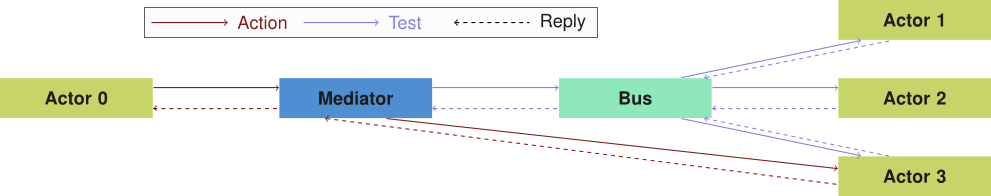
\includegraphics[width=0.5\linewidth]{images/comunica-actor-mediator-bus.png}
    \caption{Actor-Mediator-Bus patroon, foto van ``Comunica: a Modular SPARQL Query Engine for the Web'' \cite{taelman2018comunica}.}
    \label{fig:actor-mediator-bus}
\end{figure}



\subsection{Conclusie}
Om tot een besluit te komen over Comunica kunnen er enkele feiten vastgesteld worden. Eerst en vooral kan er veel uitleg gegeven worden, maar is er gepoogd om de werking ervan duidelijk te maken op een korte, doch krachtige manier. Om de volledige en uitgebreide werking en analyse van Comunica te lezen kan best doorverwezen worden naar de officiële paper: ``Comunica: a Modular SPARQL Query Engine for the Web''. De belangrijkste punten om te onthouden zijn de vijf doelen die voor ogen gesteld werden bij het maken van Comunica:
\begin{enumerate}
    \item \textbf{\textit{SPARQL query evaluation}}: het moet mogelijk zijn om SPARQL queries op een correcte manier te interpreteren en een resultaat weer te geven.
    \item \textbf{Modulair}: nieuwe functionaliteiten (of bestaande functionaliteiten aanpassen) zou slechts een minimale aanpassing aan bestaande code mogen vereisen. Hierbij kan de gebruiker zelf kiezen welke modules hij wil inpluggen voor zijn persoonlijke \textit{engine}.
    \item \textbf{Heterogene \textit{interfaces}}: de mogelijkheid om te queryen naar verschillende soorten bronnen (zoals \acrshort{tpf} \textit{interfaces}, SPARQL \textit{endpoints} en data dums in RDF) moet mogelijk zijn.
    \item \textbf{\textit{Federation}}: het moet mogelijk zijn om gefedereerd te queryen. Dit betekent queryen naar verschillende bronnen. In samenhang met de heterogene \textit{interfaces} betekent dit dus queryen naar verschillende bronnen die mogelijks een soort \textit{interface} hebben.
    \item \textbf{Web gebaseerd}: Comunica is gemaakt met web technologieën zoals Javascript en RDF configuratie bestanden. Hierdoor kan Comunica werken in omgevingen zoals \textit{web browsers}, \textit{local} en zelfs in de \textit{command-line interface}.
\end{enumerate}
\newpage
\section{OGC}
\label{sec:ogc}

Voorheen werden bestaande technieken, waarop verder gewerkt wordt, beschreven. Het vervolg van deze masterproef gaat echter over het geospatiale. Dit zijn technieken die gerespecteerd en toegepast moeten worden om zo het uiteindelijke onderzoek te kunnen doen. 

OGC staat voor Open Geospatial Consortium. Dit is een wereldwijde \textit{community} die zich inzet voor het verbeteren van de manier hoe omgegaan wordt met geospatiale locatie informatie te verbeteren. Het OGC maakt standaarden om geospatiale informatie beschikbaar te stellen, zodat deze door gebruikers op een optimale en zo uniform mogelijke manier bereikt kan worden \cite{ogcdocs}.

Het OGC voorziet vele standaarden. De standaarden die relevant zijn voor deze masterproef worden hieronder besproken.

\subsection{WKT}
WKT staat voor \textit{Well-known text}. Dit is een opmaaktaal om de geometrieobjecten op een kaart te representeren. Hierbij worden de coordinaten van een positie gescheiden door een spatie (eerst de x coördinaat, daarna de y coördinaat), opeenvolgende posities binnen één structuur worden gescheiden door een komma \cite{ogcdocs}. 

De primitieve geometrieën zijn ``\textit{Point}'', ``\textit{LineString}'' en ``\textit{Polygon}''. Een ``\textit{Point}'' staat voor één exacte locatie op een kaart. Een ``\textit{LineString}'' gaat dan weer over een lijn, dit zijn dus de verbindingen tussen verschillende punten (bijvoorbeeld van punt 1 naar punt 2 en van punt 2 naar punt 3). Ten slotte is er een ``\textit{Polygon}'', wat staat voor een vlak. Hierbij heeft het OGC nog enkele andere voorwaarden opgesteld. Een ``\textit{Polygon}'' moet topologisch gesloten zijn, wat betekent dat het laatste punt hetzelfde moet zijn als het eerste. Daarbovenop kan een ``\textit{Polygon}'' bestaan uit een buitenste en binnenste lineaire ring. De buitenste ring slaat op het vlak, terwijl de binnenste ring slaat op een vlak dat uit het grotere vlak gehaald wordt. Hierbij stelt het OGC dat de locaties van de buitenste ring in tegenwijzerszin gegeven moeten zijn, terwijl deze van de binnenste ring in wijzerszin moeten staan \cite{ogcdocs}.

Een verduidelijking van primitieve geometrieën is te zien in \tableref{tab:wkt_primitives}. Hierin is het eerste punt van een figuur steeds opgevuld voor verduidelijking. Bij een ``\textit{Polygon}'' met twee ringen wordt ook direct duidelijk waarom de dubbele haken er staan.

\begin{table}[ht]
\centering
\begin{tabular}{ |l|c|p{8cm}| } 
 \hline
 \rowcolor{TableHeaderColor} Type & \multicolumn{2}{c|}{Example} \\ \hline
 
 \rowcolor{TableColor} \multirow{4.5}{*}{Point} & \raisebox{-\height+2mm}[0pt][20mm]{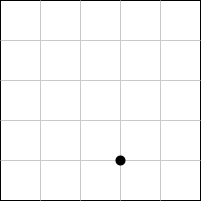
\includegraphics[width=20mm, height=20mm]{images/wkt_point.png}} & POINT (30 10) \\ \hline
 
 \rowcolor{TableColor} \multirow{4.5}{*}{LineString} & \raisebox{-\height+2mm}[0pt][20mm]{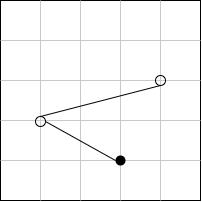
\includegraphics[width=20mm, height=20mm]{images/wkt_line.png}} & LINESTRING (30 10, 10 20, 40 30) \\ \hline
 
 \rowcolor{TableColor} & \raisebox{-\height+2mm}[0pt][20mm]{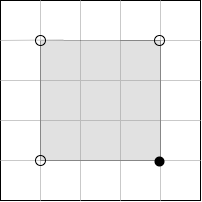
\includegraphics[width=20mm, height=20mm]{images/wkt_polygon1.png}} & POLYGON ((40 10, 40 40, 10 40, 10 10, 40 10)) \\ \cline{2-3}
 
 \rowcolor{TableColor} \multirow{-2}{*}{Polygon} & \raisebox{-\height+2mm}[0pt][20mm]{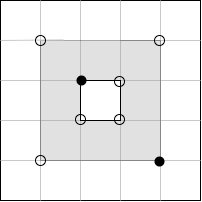
\includegraphics[width=20mm, height=20mm]{images/wkt_polygon2.png}} & POLYGON ((40 10, 40 40, 10 40, 10 10, 40 10), (20 30, 30 30, 30 20, 20 20, 20 30) \\ \hline
\end{tabular}
\caption{Primitieve geometrieën.}
\label{tab:wkt_primitives}
\end{table}

Naast de primitieve geometrieën zijn er ook de meerdelige geometrieën. Hierin bestaan ``\textit{MultiPoint}'', ``\textit{MultiLineString}'' en ``\textit{MultiPolygon}''. Deze staan respectievelijk voor één of meer van de overeenkomstige primitieve geometrieën. Ter verduidelijking van de meerdelige geometrieën is er ook een klein voorbeeld voorzien in \tableref{tab:wkt_multipart}. Hierbij gelden uiteraard dezelfde conventies als bij de primitieve geometrieën.


\begin{table}[ht]
\centering
\begin{tabular}{ |l|c|p{8cm}| } 
 \hline
 \rowcolor{TableHeaderColor} Type & \multicolumn{2}{c|}{Example} \\ \hline
 
 \rowcolor{TableColor} \multirow{4.5}{*}{MultiPoint} & \raisebox{-\height+2mm}[0pt][20mm]{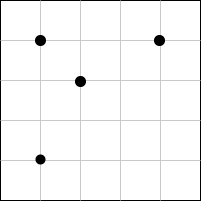
\includegraphics[width=20mm, height=20mm]{images/wkt_multipoint.png}} & MULTIPOINT ((10 40), (10 10), (20 30), (40 40)) \\ \hline
 
 \rowcolor{TableColor} \multirow{4.5}{*}{MultiLineString} & \raisebox{-\height+2mm}[0pt][20mm]{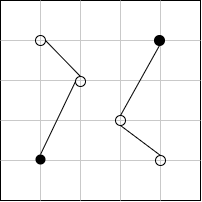
\includegraphics[width=20mm, height=20mm]{images/wkt_multiline.png}} & MULTILINESTRING ((10 10, 20 30, 10 40), (40 40, 30 20, 40 10)) \\ \hline
 
 \rowcolor{TableColor} & \raisebox{-\height+2mm}[0pt][20mm]{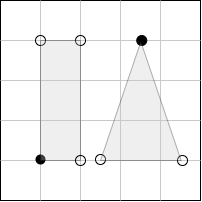
\includegraphics[width=20mm, height=20mm]{images/wkt_multipolygon1.png}} & MULTIPOLYGON (((10 10, 20 10, 20 40, 10 40, 10 10)), ((35 40, 25 10, 45 10, 35 40))) \\ \cline{2-3}
 
 \rowcolor{TableColor} \multirow{-2}{*}{MultiPolygon} & \raisebox{-\height+2mm}[0pt][20mm]{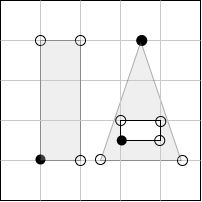
\includegraphics[width=20mm, height=20mm]{images/wkt_multipolygon2.png}} & MULTIPOLYGON (((10 10, 20 10, 20 40, 10 40, 10 10)), ((35 40, 25 10, 45 10, 35 40), (30 15, 30 20, 40 20, 40 15, 30 15))) \\ \hline
\end{tabular}
\caption{Meerdelige geometrieën.}
\label{tab:wkt_multipart}
\end{table}

\subsection{GML}
GML staat voor \textit{Geography Markup Language}. GML is een XML syntax die gedefinieerd is door het OGC met als doel om geospatiale informatie uit te drukken. GML doet dus hetzelfde als WKT, maar met andere notaties. Het is wel opmerkelijk dat het bij GML enkel mogelijk is om primitieve geometrieën te beschrijven, dus geen meerdelige geometrieën. Aangezien deze standaard minder vaak gebruikt wordt, zal deze ook minder gedetailleerd besproken worden. Zo zijn er drie verschillende manieren om coördinaten weer te geven in GML \cite{ogcdocs}:
\begin{itemize}
    \item ``<gml:coordinates>'': bij deze \textit{tag} worden de coördinaten gescheiden door een komma. Indien er meerdere locaties na elkaar komen worden deze dan weer gescheiden door een spatie.
    \item ``<gml:pos>'': bij deze \textit{tag} worden de coördinaten gescheiden door een spatie. Hier is het niet mogelijk om meerdere locaties na elkaar te laten komen.
    \item ``<gml:posList>'': deze \textit{tag} is gelijkaardig aan de ``pos'' \textit{tag}, maar hier is het wel mogelijk om meerdere locaties na elkaar te laten komen. Deze worden dan opnieuw gescheiden door een spatie.
\end{itemize}

Een kort voorbeeld van de ``posList'' notatie is te zien in \listingref{listing:gml}. Hierin wordt het voorbeeld van ``\textit{LineString}'' uit \tableref{tab:wkt_primitives} herschreven naar de GML notatie. Hierbij van het ``srsDimension'' attribuut op. Dit geeft aan hoeveel dimensies het punt heeft.

\begin{listing}[ht]
\begin{minted}{xml}
<gml:LineString gml:id="p21"
    srsName="http://www.opengis.net/def/crs/EPSG/0/4326">
    <gml:posList srsDimension="2">30 10 10 20 40 30</gml:posList>
</gml:LineString >
\end{minted}
\caption{Voorbeeld GML bij LineString.}
\label{listing:gml}
\end{listing}

\subsection{GeoSPARQL}
Ook GeoSPARQL is een standaard van het OGC. GeoSPARQL is gemaakt voor het representeren en queryen van geospatiale data op het semantische web. Zo definieert GeoSPARQL een vocabulair voor het representeren van geospatiale gegevens in RDF. Verder is het belangrijk te weten dat GeoSPARQL een uitbreiding is op de SPARQL query taal, met als doel het verwerken van geospatiale gegevens. GeoSPARQL is gemaakt om zowel systemen die gebaseerd zijn op kwalitatieve spatiale redenering als systemen die gebaseerd zijn op kwantitatieve spatiale berekeningen te huisvesten. Kortom zal GeoSPARQL nieuwe filterfuncties definiëren voor \acrfull{gis} queries (\acrshort{gis} is een informatiesysteem waarmee ruimtelijke gegevens over geografische objecten kunnen opgeslagen, beheerd, bewerkt, geanalyseerd en gerepresenteerd worden), gebruikmakend van standaarden die gedefinieerd zijn door het OGC. Dit is echter een zeer korte en beperkte uitleg over GeoSPARQL, de gedetailleerde specificatie worden toegelicht in \sectionref{sec:geosparql}.
\newpage
\section{GeoSPARQL}
\label{sec:geosparql}

Zoals eerder vermeld is GeoSPARQL één van de vele OGC standaarden. Specifieker is GeoSPARQL uitermate geschikt voor het uitvoeren van \acrshort{gis} queries, maar dit is zeker niet de enige mogelijkheid. Zoals eerder vermeld brengt GeoSPARQL een vocabulair voor de representatie van geospatiale gegevens, gebruik makend van RDF en is GeoSPARQL een uitbreiding op de SPARQL query taal. Het doel van GeoSPARQL is dan ook om geospatiale gegevens te verwerken. Voor het bekomen van een correcte implementatie van GeoSPARQL, zijn er normaliter meerdere voorwaarden waaraan de implementatie moet voldoen. De meeste van deze vereisten maken gebruik van de ``geo'', ``geof'' of ``geor'' ontologie \cite{ogcdocs}.

\subsection{Vereisten}
De vereisten zijn opgelijst in de officiële documentatie. Een samenvatting van het geheel is te vinden hieronder \cite{ogcdocs}. 
\begin{enumerate}
    \item \textbf{SPARQL}: Deze vereiste is meteen ook de belangrijkste. Deze stelt dat er een werkende implementatie van SPARQL aanwezig moet zijn. Dit betekent dat een implementatie GeoSPARQL ook alle mogelijkheden van SPARQL moet voorzien.
    \item \textbf{Klassen}: een correcte implementatie van GeoSPARQL moet de RDFS klassen ``geo: SpatialObject'', ``geo:Feature'' en ``geo:Geometry'' toestaan.
    \item \textbf{Properties}: verder moet een implementatie van GeoSPARQL ook verschillende attributen, zoals ``geo:sfContains'', ``geo:hasGeometry'' en ``geo:dimension'' naast vele andere, toestaan.
    \item \textbf{WKT}: RDFS \textit{literals} van het type ``geo:wktLiteral'' bevatten mogelijks een URI die het coördinaat stelsel van deze coördinaten beschrijft. Indien deze URI niet aanwezig is wordt er gekozen voor ``<http://www.opengis.net/def/crs/OGC/1.3/CRS84>''. Daarnaast moeten de coördinaten geïnterpreteerd worden zoals beschreven in het referentiesysteem.
    \item \textbf{GML}: naast WKT moet GML ook ondersteund worden. De implementatie moet zelf documenteren welke profielen ondersteund worden.
    \item \textbf{Functies}: Bij de implementatie van GeoSPARQL moeten meerdere functies ondersteund worden. Hierin is onderscheid gemaakt tussen topologische functies (zoals onder andere ``geof:sfContains'' en ``geof:ehContains'') en niet-topologische functies (zoals ``geof:distance'' en ``geof:union'').
    \item \textbf{Entailment}: GeoSPARQL moet dezelfde semantiek voor \textit{basic graph pattern matching} hanteren als SPARQL. Dit houdt in dat een functie als predikaat moet kunnen omgezet worden naar een query die ook functies berekent om aan een correct resultaat te komen. Hiervoor gebruikt het regels zoals onder andere ``geor:sfContains''.
\end{enumerate}

\subsection{Architectuur}
\label{subsec:geosparql_architecture}
\begin{figure}[ht]
    \centering
    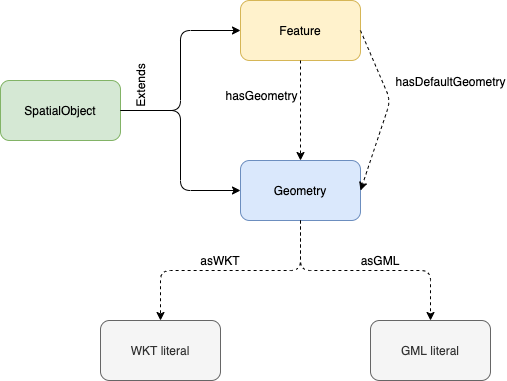
\includegraphics[width=0.5\linewidth]{images/geosparql_architecture.png}
    \caption{Vereenvoudigd diagram van de GeoSPARQL klassen ``Feature'' en ``Geometry'' met sommige properties (figuur gebaseerd op \cite{geosparqlsupport}).}
    \label{fig:geosparql_architecture}
\end{figure}

Om de architectuur vereenvoudigd weer te geven kan \figureref{fig:geosparql_architecture} helpen. Hierin is te zien dat er één hoofdklasse is waar de andere van overerven, genaamd ``SpatialObject''. Het belangrijke hier is het verschil tussen een ``Feature'' en een ``Geometry''. Een ``Geometry'' is het effectieve spatiale object, dat weergegeven kan worden als WKT of als GML (zie verder in \subsectionref{subsec:geosparql_properties}). Eén van de belangrijke (en niet vanzelfsprekende) ontwerpkeuzes is het gebruik van de ``Feature'' klasse. Deze werkt als een soort wrapper klasse voor ``Geometry''. Dit is belangrijk om te weten voor verderop in \subsectionref{subsec:geosparql_rewrite_query}, maar daar zal nogmaals terug verwezen worden naar deze subsectie.

\subsection{Properties}
\label{subsec:geosparql_properties}
GeoSPARQL voorzien een hele lijst met properties die voorzien moet worden. Vanwege de eerder korte periode om een volledige implementatie van GeoSPARQL te maken, wordt hier minder aandacht aan gegeven. Enkele voorbeelden van deze attributen zijn de volgende \cite{ogcdocs}:

\begin{itemize}
    \item \textbf{geo:isEmpty}: dit attribuut zal ``true'' terug geven indien de geometrie geen punten bevat.
    \item \textbf{geo:isSimple}: Dit attribuut zal ``true'' geven indien de geometrie geen intersecties met zichzelf bevat. Dit kan wel uitgezonderd zijn \textit{boundary} zijn.
    \item \textbf{geo:hasSerialization}: Dit attribuut wordt gebruikt om een geometrie te connecteren met zijn text-gebaseerde serialisatie. Dit kan WKT of GML zijn, maar aangezien deze uitgebreid besproken zijn in \sectionref{sec:ogc}, wordt dit hier niet herhaald. Het kan wel nogmaals benadrukt worden dat deze \textit{literal} optioneel kan bijhouden welk topologisch referentiesysteem gebruikt wordt. Het is wel belangrijk te weten waarom deze referentiesystemen zo belangrijk zijn. Australië bijvoorbeeld, verdrijft jaarlijks wat van zijn oorspronkelijke locatie. Na een aantal jaar zou elk huis op de kaart een volledig huis verder liggen, waardoor de informatie nutteloos geworden is. GeoSPARQL lost dit op met het gebruik van de referentiesystemen.
\end{itemize}


\subsection{Topologische relaties}
\label{subsec:topologische_relaties}
Om topologische relaties te kunnen beschrijven, wordt er gebruik gemaakt van drie relatiefamilies. Deze relatiefamilies beschrijven grotendeels gelijkaardige topologische relaties, maar met licht verschillende specificaties. De drie relatiefamilies zijn ``Simple Features (sf)'', ``Egenhofer (eh)'' en ``RCC8''. Om de spatiale relaties te beschrijven wordt gebruik gemaakt van een ``DE-9IM'' patroon. Voordat de relatiefamilies uitgelegd kunnen worden, is een volledig begrip van de DE-9IM notatie noodzakelijk.

\subsubsection{DE-9IM}
\begin{figure}[ht]
    \centering
    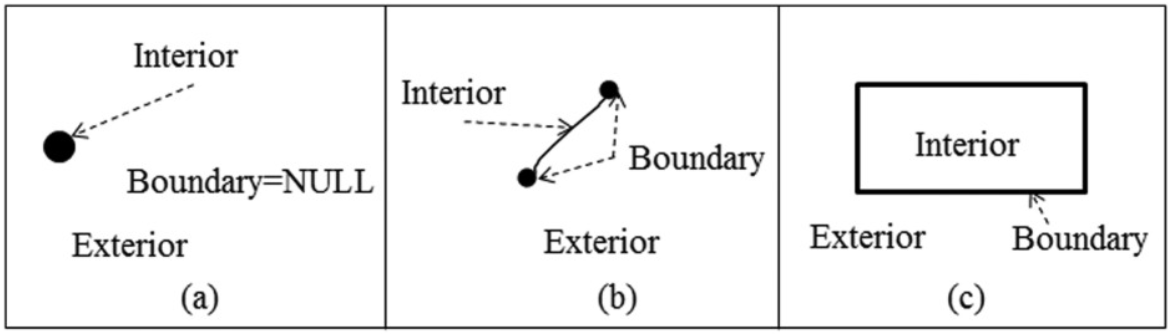
\includegraphics[width=0.9\linewidth]{images/spatial_objects_DE-9IM.png}
    \caption{Spatiale objecten met hun \textit{interior}, \textit{boundary} en \textit{exterior}: (a) Een punt; (b) Een lijn; (c) Een vlak. Figuur van \cite{shen2018classification}}.
    \label{fig:de-9im}
\end{figure}

DE-9IM staat voor \textit{Dimensionally Extended Nine-Intersection Model}. Dit model kan afgebeeld worden als een 3x3 matrix, waarbij (in deze volgorde) de \textit{interior}, \textit{boundary} en \textit{exterior} van het ene spatiale object vergeleken wordt met deze van het andere spatiale object. Deze matrix geeft de dimensies van de intersectie van deze objecten weer. De betekenis van \textit{interior}, \textit{boundary} en \textit{exterior} voor de verschillende soorten spatiale objecten is verduidelijkt in \figureref{fig:de-9im}. De volledige 3x3 matrix voor de objecten a en b is van de volgende vorm \cite{shen2018classification}:

\begin{equation*}
    DE-9IM(a,b) = 
    \begin{bmatrix}
    dim(I(a)\cap I(b)) & dim(I(a)\cap B(b)) & dim(I(a)\cap E(b))\\
    dim(B(a)\cap I(b)) & dim(B(a)\cap B(b)) & dim(B(a)\cap E(b))\\
    dim(E(a)\cap I(b)) & dim(E(a)\cap B(b)) & dim(E(a)\cap E(b))
    \end{bmatrix}
\end{equation*}

\begin{figure}[ht]
    \centering
    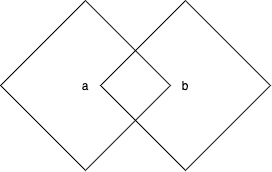
\includegraphics[width=0.5\linewidth]{images/de-9im_example.png}
    \caption{Voorbeeld voor de DE-9IM matrix.}
    \label{fig:de-9im_example}
\end{figure}

Wanneer dit toegepast wordt op de objecten die te zien zijn in \figureref{fig:de-9im_example}, dan wordt de volgende matrix bekomen:

\begin{equation*}
    DE9IM(a,b) = 
    \begin{bmatrix}
    2 & 1 & 2\\
    1 & 0 & 1\\
    2 & 1 & 2
    \end{bmatrix}
\end{equation*}

Voor het bepalen van de relaties van de GeoSPARQL families zijn er echter nog iets andere regels opgesteld. Hier heeft het OGC nieuwe betekenissen geïntroduceerd: 
\begin{enumerate}
    \item \textbf{Empty}: dit wordt genoteerd als -1.
    \item \textbf{True}: Dit geldt wanneer de waarden 0, 1, 2 voorkomen. Bij deze waarde kan soms gespecifieerd worden dat het een bepaalde waarde exact moet uitkomen. Het kan ook genoteerd worden als ``T'' (dit is trouwens meer wel dan niet het geval).
    \item \textbf{False}: dit geldt wanneer de waarde -1 wordt uitgekomen, maar wordt genoteerd als ``F''.
    \item \textbf{Don't care}: Dit betekent dat eender welke waarde mag voorkomen en dat dit hier niet naar gekeken moet worden. Dit wordt genoteerd als ``*''.
\end{enumerate}
Hierbij wordt het patroon geschreven als een sequentie van negen karakters. Als deze van links naar rechts gelezen wordt, dan stelt dit de DE-9IM matrix voor van linksboven beginnend, rij per rij opvullend. Het volgende patroon staat dus voor de overeenkomstige matrix:

\begin{equation*}
    T**T**T** = 
    \begin{bmatrix}
    T & * & *\\
    T & * & *\\
    T & * & *
    \end{bmatrix}
\end{equation*}
Indien er meer dan één lijn staat, wil dit zeggen dat één van de mogelijke matrices voldoende is om te besluiten dat de relatie klopt.

Ten slotte kunnen ook niet alle relaties voorkomen bij elke object-combinatie (bijvoorbeeld twee punten kunnen elkaar niet kruisen). Daarom wordt er ook een nieuwe notatie toegevoegd in de GeoSPARQL-documentatie, om te vermelden op welke spatiale objecten het DE-9IM intersectie patroon van toepassing is. Hierbij staat symbool ``P'' voor 0-dimensionale geometrieën (zoals punten). Het symbool ``L'' staat dan weer voor 1-dimensionale geometrieën (zoals lijnen). Het laatste symbool is ``A'', wat dan weer staat voor 2-dimensionale geometrieën (zoals vlakken) \cite{ogcdocs}.


\subsubsection{Simple Features}
\label{subsubsec:simple_features}
De eerste relatiefamilie is de ``Simple Feature'' family. De regels van deze familie worden weergegeven in \tableref{tab:topo_sf}. Hierin is exact te zien hoe de implementaties verwacht worden te werken. Om de grootte van deze masterproef in te perken is enkel deze relatiefamilie uitgewerkt en wordt dus ook enkel deze relatiefamilie besproken. Indien het voorbeeld van de ``contains'' functie besproken wordt, moet dit als volgt geïnterpreteerd worden: ``a contains b is waar, indien de intersectie van hun \textit{interiors} bestaat en hierbovenop de intersectie van de \textit{exterior} van a met zowel de \textit{interior} als de \textit{boundary} van b niet bestaat''. Dit betekent dus dat b in a ligt en dat geen enkel deel van b buiten a ligt \cite{ogcdocs}.


\begin{table}[ht]
    \centering
    \begin{tabular}{ |p{1.5cm}|l|l|p{2cm}|p{2.5cm}| } 
        \hline
        \rowcolor{TableHeaderColor} Relation Name & Relation URI & Domain/Range & Applies To Geometry Types & DE-9IM Intersection pattern \\ \hline
        
        \rowcolor{TableColor} equals & geo:sfEquals & geo:SpatialObject & All & (TFFFTFFFT) \\ \hline
        
        \rowcolor{TableColor} disjoint & geo:sfDisjoint & geo:SpatialObject & All & (FF*FF****) \\ \hline
        
        \rowcolor{TableColor} intersects & geo:sfIntersects & geo:SpatialObject & All & (T********
        *T*******
        ***T*****
        ****T****)  \\ \hline
        
        \rowcolor{TableColor} touches & geo:sfTouches & geo:SpatialObject & All except P/P & (FT*******
        F**T*****
        F***T****) \\ \hline
        
        \rowcolor{TableColor} within & geo:sfWithin & geo:SpatialObject & All & (T*F**F***) \\ \hline
        
        \rowcolor{TableColor} contains & geo:sfContains & geo:SpatialObject & All & (T*****FF*) \\ \hline
        
        \rowcolor{TableColor} overlaps & geo:sfOverlaps & geo:SpatialObject & A/A, P/P, L/L & ((T*T***T**)
        for A/A, P/P;
        (1*T***T**)
        for L/L) \\ \hline
        
        \rowcolor{TableColor} crosses & geo:sfCrosses & geo:SpatialObject & P/L, P/A, L/A, L/L & ((T*T***T**)
        for P/L, P/A,
         L/A;
        (0********)
        for L/L) \\ \hline
        
    \end{tabular}
    \caption{Simple Features Topological Relations (tabel van \cite{ogcdocs}).}
    \label{tab:topo_sf}
\end{table}


\subsection{Niet-topologische relaties}

Verder zijn er ook de niet-topologische relaties. Verschillende van deze functies gebruiken een meeteenheid URI. Daarom heeft het OGC enkele standaard meeteenheden gedefinieerd, te vinden onder de \textit{namespace} ``http://www.opengis.net/def/uom/OGC/''. Een voorbeeld van zo een meeteenheid is ``<http://www.opengis.net/def/uom/OGC/metre>''. Enkele van de niet-topologische functies zijn de volgende: \cite{ogcdocs}.

\begin{itemize}
    \item \textbf{geof:distance}: deze functie moet de kortst mogelijke afstand geven tussen twee objecten.
    \item \textbf{geof:buffer}: deze functie geeft een geometrie terug die alle punten bevat die binnen een bepaalde radius van een meegegeven geometrie liggen.
    \item \textbf{geof:convexHull}: deze functie geeft een geometrie terug die het kleinste convexe omhulsel is dat alle punten omvat van een meegegeven geometrie.
    \item \textbf{geof:intersection}: deze functie geeft een geometrie terug die staat voor alle punten van de intersectie tussen twee geometrieën.
    \item \textbf{geof:union}: deze functie geeft een geometrie terug die staat voor alle punten in de unie van twee geometrieën.
    \item \textbf{geof:envelope}: Deze functie geeft de minimaal omvattende (\textit{bounding}) \textit{box} weer voor een geometrische figuur. Dit betekent dus de kleinst mogelijke rechthoek waar elk punt van de geometrie in zit.
    
\end{itemize}

Ten slotte is het belangrijk te vermelden dat alle berekeningen horen te gebeuren in het referentiesysteem van de eerste geometrie die meegegeven is aan een functie, zowel bij topologische als niet-topologische functies \cite{ogcdocs}.


\subsection{Query Rewrite Extension}
\label{subsec:geosparql_rewrite_query}
De laatste uitdaging is het probleem waar de topologische functies als predikaat staan. Hierbij zou verwacht worden dat deze op voorhand berekend zijn en zo opgeslagen zijn in de RDF dataset. Hierbij is echter het probleem dat wanneer dit niet op voorhand berekend is, men nog steeds de correcte oplossing wil. Wanneer een deel van de gegevens uit de ene dataset komt en het andere deel uit een andere bron, zelfs dan wordt een correct antwoord verwacht, hoewel hier geen optie is tot het op voorhand uitrekenen \cite{ogcdocs}. 

Hiervoor wordt gebruik gemaakt van de \textit{query rewrite} uitbreiding. Deze techniek zal de query uitbreiden, door de unie (de SPARQL \textit{union}, niet de niet-topologische functie van GeoSPARQL!) te nemen van de oorspronkelijke stelling met enerzijds de relatie als predikaat en anderzijds het nieuwe uitgebreide deel waarbij dezelfde relatie uitgerekend wordt als functie. Hierbij is het ook belangrijk rekening te houden met het verschil tussen een ``Feature'' en een ``Geometry'' (zoals uitgelegd in \subsectionref{subsec:geosparql_architecture}), waardoor er vier extra delen nodig zijn voor de mogelijke combinaties tussen ``Feature'' en ``Geometry'' \cite{ogcdocs}. 

Zo heeft het OGC een template gemaakt om dit te herschrijven. Bij deze template zijn er een aantal placeholders gebruikt \cite{ogcdocs}:
\begin{itemize}
    \item \textbf{ogc:relation}: deze placeholder staat voor de relatie die gebruikt wordt (dit zou bijvoorbeeld de ``geo:sfContains'' kunnen zijn).
    \item \textbf{ogc:function}: deze placeholder staat voor de overeenkomstige functie bij de relatie die gebruikt wordt (in het voorbeeld van ``geo:sfContains'' zou de functie ``geof:sfContains'' zijn).
    \item \textbf{ogc:asGeomLiteral}: deze placeholder staat voor één van de serialisatie technieken om het object te bekomen.
\end{itemize}

Een voorbeeld voor het herschrijven van een query is te vinden in \listingref{listing:geosparql_query_to_rewrite}, maar de uiteindelijke template voor het herschrijven van de query is te vinden in \listingref{listing:geosparql_rewrite_query}.

\begin{listing}[ht]
    \begin{minted}{sparql}
        select *
        where {
            { ?f1 ogc:relation ?f2 . }
        }
    \end{minted}
    \caption{Query to rewrite.}
    \label{listing:geosparql_query_to_rewrite}
\end{listing}

\begin{listing}[ht]
    \begin{minted}{sparql}
        select *
        where {
            { ?f1 ogc:relation ?f2 . }
            UNION
            # feature - feature rule
            {   ?f1 geo:hasDefaultGeometry ?g1 . 
                ?f2 geo:hasDefaultGeometry ?g2 .
                ?g1 ogc:asGeomLiteral ?g1Serial .
                ?g2 ogc:asGeomLiteral ?g2Serial .
                filter(ogc:function(?g1Serial, ?g2Serial)) }
            UNION
            # feature - geometry rule
            {   ?f1 geo:hasDefaultGeometry ?g1 . 
                ?g1 ogc:asGeomLiteral ?g1Serial .
                ?f2 ogc:asGeomLiteral ?g2Serial .
                filter(ogc:function(?g1Serial, ?g2Serial)) }
            UNION
            # geometry - feature rule
            {   ?f2 geo:hasDefaultGeometry ?g2 .
                ?f1 ogc:asGeomLiteral ?g1Serial .
                ?g2 ogc:asGeomLiteral ?g2Serial .
                filter(ogc:function(?g1Serial, ?g2Serial)) }
            UNION
            # geometry - geometry rule
            {   ?f1 ogc:asGeomLiteral ?g1Serial .
                ?f2 ogc:asGeomLiteral ?g2Serial .
                filter(ogc:function(?g1Serial, ?g2Serial)) }
        }
    \end{minted}
    \caption{Query rewrite template (listing van \cite{ogcdocs}).}
    \label{listing:geosparql_rewrite_query}
\end{listing}
\newpage
\chapter{Implementatie}
\label{chap:implementatie}
Om de hypothesen (\sectionref{sec:onderzoeksvraag}) af te toetsen, moet er een werkende implementatie zijn van GeoSPARQL. De structuur van dit hoofdstuk zal dezelfde volgorde aannemen als hoe de implementatie is verlopen. Dit toont een zekere structuur, zodat elk deel steeds onmiddellijk getest kan worden. 


\section{Comunica}
\label{sec:impl_comunica}
Zoals eerder aangehaald speelt Comunica een zeer belangrijke rol bij deze implementatie van GeoSPARQL (zie \sectionref{sec:comunica}). Hierbij (dankzij de modulariteit) is het mogelijk om een actor aan te maken voor het afhandelen van GeoSPARQL-functionaliteiten. Deze actor maakt gebruik van ``sparqlalgebrajs'' om de SPARQL query om te vormen naar SPARQL algebra en van ``sparqlee'' om deze SPARQL algebra correct uit te werken. 

\subsection{Sparqlalgebrajs}
\begin{listing}[ht]
    \begin{minted}{sparql}
        SELECT ?f
        WHERE {
            my:A my:hasExactGeometry ?aGeom .
            ?aGeom geo:asWKT ?aWKT .
            ?f my:hasExactGeometry ?fGeom .
            ?fGeom geo:asWKT ?fWKT .
            FILTER (geof:sfContains(?aWKT, ?fWKT) && !sameTerm(?aWKT, ?fWKT))
        }
    \end{minted}
    \caption{Example SPARQL query.}
    \label{listing:sparqlalgebrajs_query}
\end{listing}

\begin{listing}[ht]
    \begin{minted}{json}
        {
        ...,
        expression: {
            type: 'expression',
            expressionType: 'operator',
            operator: '&&',
            args: [
            {
                type: 'expression',
                expressionType: 'named',
                name: NamedNode {
                id: 'http://www.opengis.net/def/function/geosparql/sfContains'
                },
                args: [
                {
                    type: 'expression',
                    expressionType: 'term',
                    term: Variable { id: '?aWKT' }
                },
                {
                    type: 'expression',
                    expressionType: 'term',
                    term: Variable { id: '?fWKT' }
                }
                ]
            },
            {
                type: 'expression',
                expressionType: 'operator',
                operator: '!',
                args: [
                {
                    type: 'expression',
                    expressionType: 'operator',
                    operator: 'sameterm',
                    args: [
                    {
                        type: 'expression',
                        expressionType: 'term',
                        term: Variable { id: '?aWKT' }
                    },
                    {
                        type: 'expression',
                        expressionType: 'term',
                        term: Variable { id: '?fWKT' }
                    }
                    ]
                }
                ]
            }
            ]
        }
        }
    \end{minted}
    \caption{Example SPARQL algebra.}
    \label{listing:sparqlalgebrajs_algebra}
\end{listing}

Sparqlalgebrajs zorgt er onder andere voor dat de filter omgezet wordt naar een boomstructuur die recursief kan worden doorlopen. Deze omvorming is te zien in \listingref{listing:sparqlalgebrajs_query} en \listingref{listing:sparqlalgebrajs_algebra}. In \listingref{listing:sparqlalgebrajs_query} is een voorbeeld van een correct GeoSPARQL query te zien (ter informatie: deze query haalt alle vormen in die geografisch in ``my:A'' liggen, maar niet ``my:A'' zelf zijn), maar voor het uitvoeren van deze query moet deze eerst omgevormd worden naar SPARQL algebra. Vanwege de grootte van het resultaat is slechts de essentie hiervan terug te vinden in \listingref{listing:sparqlalgebrajs_algebra}. Aangezien het gaat over de filterfunctie, is enkel dat deel terug te vinden. Hierbij is zeer duidelijk de recursieve boomstructuur te vinden, waarbij in de wortel van de boom de operator ``\&\&'' te zien is. Dit blad in de boom zal vervolgens een linker- en rechterkind hebben. Deze zijn te vinden in het veld ``args'' en krijgen de waarde van opnieuw de uitkomst van twee bladeren. Ditmaal zijnde de ``sfContains'' functie aan de linker helft en de ``!'' operator aan de rechter helft. Dit wordt op deze manier recursief uitgevoerd.

\subsection{Sparqlee}
Sparqlee is een SPARQL \textit{expression evaluator}. Dit betekent dat sparqlee een SPARQL algebra expressie zal evalueren. Sparqlee is bij deze implementatie gebruikt voor het maken van de GeoSPARQL functionaliteiten, omdat sparqlee zelf als de recursieve boomstructuur van sparqlalgebrajs volledig afhandelt voor SPARQL queries. Dit is belangrijk voor de belangrijkste vereiste voor GeoSPARQL, namelijk het hebben van een werkende SPARQL implementatie. Zo zal sparqlee eerst de volledige expressie controleren om te zien of het geheel verwerkt kan worden. Dit is dus enkel het geval als sparqlee de verschillende functies en operators correct kan afhandelen. In dit specifieke geval betekent het dus dat sparqlee de GeoSPARQL functies moet kunnen uitvoeren. Hiervoor is dezelfde programmeerstijl gehanteerd als deze die al aanwezig is in sparqlee zelf.

\subsection{Verbeteringen}
Een eerste verbetering aan deze eerste keuze is meteen dat deze GeoSPARQL functies niet in sparqlee gemaakt zouden mogen worden. Sparqlee is louter een SPARQL \textit{expression evaluator}, wat betekent dat deze niet meer dan enkel SPARQL hoort te ondersteunen. De oplossing hiervoor is het ondersteunen van \textit{custom functions} binnen sparqlee (dit staat bovendien binnen de specificaties van SPARQL). Indien deze \textit{custom functions} ondersteund zouden worden binnen sparqlee, dan zou het mogelijk zijn om de functies te implementeren binnen de hiervoor gemaakte actor in Comunica. Op deze manier kan deze dan geïnjecteerd worden in sparqlee. Het implementeren van deze \textit{custom functions} functionaliteit binnen sparqlee is echter te complex en tijdrovend voor de eerder kleine impact op deze masterproef. Dit blijft echter wel een vereiste voor de modulariteit, maar dit wordt gezien als \textit{future work}. 
\newpage
\section{Datastructuur}
\label{sec:datastructuur}
Voordat begonnen kan worden aan de effectieve oplossing van GeoSPARQL functies, moet de gepaste datastructuur gekozen worden om dit te kunnen realiseren. Zoals beschreven in \sectionref{subsec:geosparql_architecture}, moet er ondersteuning zijn voor zowel ``Geometry'' als ``Feature'' objecten. 

\subsection{GeoJSON}
Om dit te kunnen ondersteunen is er gekozen voor een vaker gebruikt formaat, genaamd GeoJSON. GeoJSON biedt ondersteuning voor zowel ``Geometry'' als ``Feature'' objecten, waarbij ``Feature'' objecten een ``Geometry'' object bevatten, naast andere attributen. Bovendien ondersteunt GeoJSON de volgende vormen: ``Point'', ``LineString'', ``Polygon'', ``MultiPoint'', ``MultiLineString'' en ``MultiPolygon''. Op deze manier zijn alle voorwaarden van de architectuur voor GeoSPARQL voldaan. Het volgende probleem is dan: hoe kan een WKT string omgevormd worden naar GeoSPARQL?

\subsection{Terraformer}
Terraformer is een geografische toolkit voor het werken met onder andere geometrieën, geografie en formaten. Verder is Terraformer opgesplitst in enkele modules. Hier wordt verder (zie \sectionref{sec:topologische_functies}) op terug gekomen. Voorlopig wordt enkel verder ingegaan op de Terraformer WKT parser. Deze module is gemaakt om te voorzien in een eenvoudige omzetting van WKT string naar GeoJSON en indien gewenst ook in de omgekeerde richting. Op deze manier kan een geserialiseerde vorm (namelijk WKT string) omgezet worden naar GeoJSON, zodat nu verder gegaan kan worden met de implementatie. 



 
\newpage
\section{Topologische functies}
\label{sec:topologische_functies}
Een van de belangrijkste functionaliteiten van GeoSPARQL is het topologisch van elkaar kunnen onderscheiden van vormen. Hiervoor zijn er drie verschillende relatiefamilies (zoals eerder aangehaald, zie \subsectionref{subsec:topologische_relaties}). Vanwege de eerder korte periode voor deze masterproef is ervoor gekozen om de focus te leggen op slechts één van deze families, namelijk de ``Simple Features'' familie. Om niet te vaak in herhaling te vallen kan best terugverwezen worden naar \subsubsectionref{subsubsec:simple_features} om te kijken naar de specificaties van deze familie. Om de eerste functie te maken is gekozen voor de ``sfContains'' functie. De \textit{contains}-functie is een veel gebruikte en voor de hand liggende functie, die gaat controleren of een vorm binnen een andere vorm ligt. Om de verschillende functies te testen werd een eenvoudige testset gecreëerd. Deze testset is te zien in \figureref{fig:illustration_spatial_data}. Om tot een eerste uitkomst te komen, was er al een zeer goede oplossing. Dit bleek Terraformer te zijn.

\begin{figure}[ht]
    \centering
    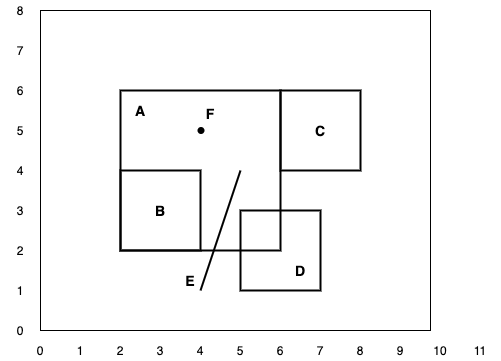
\includegraphics[width=0.5\linewidth]{images/geosparql_example.png}
    \caption{Illustratie geospatiale data van \cite{ogcdocs}}
    \label{fig:illustration_spatial_data}
\end{figure}

\subsection{Terraformer}
Terraformer was een eerste en zeer voor de hand liggende keuze, omdat deze reeds gebruikt werd voor de omzetting van WKT naar GeoJSON. Zo heeft Terraformer een module voor het werken met GeoJSON. De module heet Terraformer Core. Deze module voorziet functies voor onder andere het controleren of een vorm binnen een andere vorm ligt en om te controleren of een vorm een andere vorm snijdt. Dit is welliswaar te beperkt om de volledige ``Simple Features'' familie te implementeren, maar voor de ``sfContains'' en nadien voor zowel de ``sfIntersects'' en de ``sfDisjoint'' functies is dit zeker een goed begin. 

Na het maken van de implementatie, bleken er toch enkele problemen te zijn met de ``contains'' functie van Terraformer. Zo valt onmiddellijk op dat er vele randgevallen zijn die niet correct werken. Enkele voorbeelden daarvan zijn de volgende:
\begin{itemize}
    \item Polygoon ``contains'' lijn: wanneer de lijn van een hoekpunt naar een ander hoekpunt gaat (dus wanneer het een zijde of een diagonaal is), zou dit ``true'' moeten geven, maar dit geeft ``false''.
    \item Polygoon ``contains'' polygoon: wanneer de polygonen een hoekpunt delen (dus deze ligt erin, maar ligt helemaal in de hoek), zou dit ``true'' moeten geven, maar dit geeft ``false''.
\end{itemize}

Om, gebruik makend van Terraformer, deze problemen op te lossen zou teveel code aangepast moeten worden. Aangezien deze randgevallen zeer vaak voorkomen (en aangezien de kans reëel is dat er nog meerdere andere fouten zijn), werd besloten om een andere oplossing te zoeken die meer bruikbaar is voor het geheel, zoals de andere topologische functies.

\subsection{Manueel}
Het eerstvolgende idee was om dit manueel op te lossen. Dit leek een logische oplossing, omdat zo alle functies met zekerheid gemaakt kunnen worden en dit met een implementatie die conform is met de OGC-standaarden. Hier werd echter vrij snel van afgeweken vanwege de complexiteit. Het uitgevoerde onderzoek wordt hieronder beschreven, opnieuw voor het voorbeeld van de ``contains'' functie. Hierbij werd ook enkel aandacht gegeven aan de enkelvoudige vormen (dus ``Point'', ``LineString'' en ``Polygon''). De gedachtengang hierbij was dat de meervoudige vorm identiek was, maar zich meerdere keren herhaalt.

\subsubsection{Point}
Bij het beginnen van een eigen implementatie is het eenvoudigste om te beginnen bij een punt. Hierbij is het namelijk zo dat een punt enkel in een punt ligt wanneer dit punt exact hetzelfde is. Het controleren of een lijn of een polygoon in een punt ligt is nog eenvoudiger, dit is namelijk niet mogelijk (en bijgevolg dus altijd ``false'').  

\subsubsection{LineString}
Het volgende deel is logischerwijs controleren wat binnen een lijn kan liggen. Voor een punt is dit wiskundig eenvoudig op te lossen, door voor elk deel van de lijn de richtingscoëfficient uit te rekenen en vervolgens te kijken of het punt op de lijn ligt. Hierbij moet wel opgelet worden, aangezien het deel van de lijn niet oneindig doorloopt. Dit is evenwel eenvoudig op te lossen door te controleren dat de x-coördinaat van het punt tussen de x-coördinaten van de uiteinden van de lijn ligt.

Bij het controleren of een lijn in een andere lijn ligt, kan dezelfde techniek als bij een punt gebruikt worden. Hierbij moet voor elk deel van de mogelijks binnen liggende lijn gecontroleerd worden of de uiteinden op de eerste lijn liggen. Ook moet er gecontroleerd worden of de richtingscoëfficient van beide lijnen in dit deel (het volledige deel) identiek is. Indien deze voorwaarden voldaan zijn, dan ligt de lijn binnen de andere lijn. 

De controle of een polygoon binnen een lijn ligt is overbodig. Dit is namelijk onmogelijk, bijgevolg kan deze functie rechtstreeks ``false'' als uitkomst geven.

\subsubsection{Polygon}
Het laatste en moeilijkste deel is controleren of een vorm binnen een polygoon ligt. Het eerste deel is het controleren of een punt binnen een polygoon ligt. Intuïtief wordt direct gedacht aan het wiskundig beschrijven van een vlak, maar dit is echter niet bruikbaar. Vervolgens kan gecontroleerd worden of het punt onder of boven een lijn ligt, om zo te proberen achterhalen of dit betekent dat het punt binnen de polygoon ligt. Het probleem heeft echter een eenvoudigere oplossing dan dit. Wanneer het punt op een lijn van de polygoon ligt, is meteen geweten dat de ``contains'' functie ``true'' moet weergeven. Wanneer dit niet het geval is, kan een andere techniek gebruikt worden. Zo kan een horizontale lijn getrokken worden, vertrekkend vanuit het punt en helemaal naar rechts (met oneindige lengte). Wanneer nu geteld wordt met hoeveel lijnen van de polygoon deze lijn kruist, is de uitkomst gekend. Het punt ligt namelijk binnen de polygoon wanneer het aantal kruissende lijnen een oneven aantal is. Deze techniek is geïllustreerd in \figureref{fig:polygon_contains_point}.

\begin{figure}
    \centering
    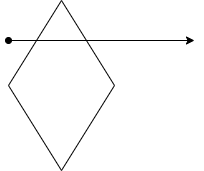
\includegraphics[width=0.5\linewidth]{images/polygon_contains_point.png}
    \caption{Voorbeeld polygon contains point.}
    \label{fig:polygon_contains_point}
\end{figure}

Het volgende deel is het controleren of een lijn binnen een polygoon ligt. Hiervoor is er opnieuw een techniek. Voor de lijn moet gecontroleerd worden of een punt binnen de polygoon ligt. Indien dit het geval is, moet ook nog eens gecontroleerd worden of de lijn snijdt met een rand van de polygoon. Dit betekent dat elke lijn van de rand van de polygoon gecontroleerd moet worden. Het controleren of lijnen snijden is opnieuw wiskundig aan te pakken, maar hier wordt niet verder op ingegaan. Deze techniek is geïllustreerd in \figureref{fig:polygon_contains_line}.

\begin{figure}
    \centering
    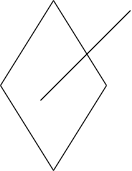
\includegraphics[width=0.3\linewidth]{images/polygon_contains_line.png}
    \caption{Voorbeeld van polygon contains line.}
    \label{fig:polygon_contains_line}
\end{figure}

Het laatste deel hierbij is het controleren of een polygoon binnen een polygoon ligt. Hiervoor zou intuïtief gedacht kunnen worden aan het controleren of alle punten van de (vermoedelijk) binnenste polygoon binnen de andere polygoon liggen. Zoals geïllustreerd in \figureref{fig:polygon_contains_polygon} is dit niet altijd het geval. Dit is enkel mogelijk indien de buitenste vorm convex (= bolvormig) is. Aangezien dit in vele gevallen niet zo is, zou het verlies van performantie zijn om hierop te controleren. Een correcte techniek is echter controleren of één enkel punt van de (vermoedelijk) binnenste polygoon binnen de andere polygoon ligt. Vervolgens volstaat het om te controleren of er een lijn van de rand van de ene polygoon snijdt met een lijn van de rand van de andere polygoon. Indien er snijdende lijnen zijn, zal de ``contains'' functie ``false'' teruggeven. Hierbij wordt ook duidelijk dat deze berekeningen computationeel intensief worden, zeker in het geval van queryen. Dit kan nog verbeterd worden door de lijnintersectietests te versnellen met het ``\textit{sweep line}'' algoritme, maar hier wordt niet verder op ingegaan. In het voorbeeld in \figureref{fig:polygon_contains_polygon} is de gekleurde polygoon diegene die getest wordt om binnen de andere te liggen.

\begin{figure}
    \centering
    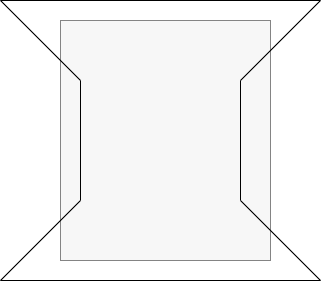
\includegraphics[width=0.3\linewidth]{images/polygon_contains_polygon.png}
    \caption{Voorbeeld van polygon contains polygon.}
    \label{fig:polygon_contains_polygon}
\end{figure}


\subsubsection{Extra moeilijkheden}
De eerder vernoemde technieken zijn al vrij ingewikkeld en dit is slechts voor de ``contains'' functie. Hier zouden nog meerdere andere technieken gebruikt moeten worden om de andere functies te implementeren. Dit wordt nog ingewikkelder wanneer ook rekening gehouden wordt met de veelvoudige vormen zoals ``MultiPoint'', ``MultiLineString'' en ``MultiPolygon''. Hierbovenop is er ook nog geen rekening gehouden met de binnenste ring van de polygonen, die een deel van het vlak excluderen. Dit is nog een extra moeilijkheidsfactor waar rekening mee moet worden gehouden.  

Zo zijn er vele nadelen aan het zelf implementeren hiervan. Een eigen implementatie bevat snel fouten bij de vereiste functionaliteiten zoals ze hierboven beschreven werden. Ook moet dit uitvoerig getest worden, wat best door een maximaal aantal gebruikers gebeurt. Bovendien moeten de meest performante algoritmes gebruikt worden, zodat dit bruikbaar is voor queries. Al deze redenen verwerpen het zelf implementeren. Daarom werd ervoor gekozen om overgegaan ``Turf.js'' te gebruiken.

\subsection{Turf.js}
``Turf.js'' is een modulaire geospatiale engine die gemaakt is in JavaScript. Zo is Turf een JavaScript \textit{library} die werkt aan de hand van GeoJSON. Het is een verzameling van kleine modules, zodat gebruik kan gemaakt worden van exact wat nodig is voor de \textit{use case}. Turf gebruikt naar eigen zeggen de nieuwste algoritmes, wat een pluspunt is voor de performantie. Bovendien heeft Turf een uitgebreide \textit{community}, wat ervoor zorgt dat mogelijke fouten in de implementatie gevonden en opgelost worden. Zo kan een bug opgelost worden door de nieuwste versie binnen te halen.

Turf voorziet vele methoden om te gebruiken in eigen berekeningen. Daarnaast heeft Turf al enkele \textit{build in} functies, zoals ``booleanContains'', ``booleanDisjoint'' en ``booleanOverlap''. Deze functies zijn exact wat nodig is. Een overzicht van de functies die gebruikt zijn voor de implementatie van de ``Simple Features'' familie is te zien in \tableref{tab:turf_functions}.

\begin{table}[ht]
    \centering
    \begin{tabular}{ |p{2cm}|p{2cm}|p{8cm}| } 
        \hline
        \rowcolor{TableHeaderColor} GeoSPARQL functie & Turf.js functie & Opmerkingen \\ \hline
        
        \rowcolor{TableColor} sfEquals & booleanEqual & De functie van Turf is volledig conform met de documentatie. \\ \hline

        \rowcolor{TableColor} sfDisjoint & booleanDisjoint & De functie van Turf blijkt volledig conform te zijn met de documentatie van GeoSPARQL. Deze bevat echter een bug waarbij twee evenwijdige en overlappende lijnen toch ``disjoint'' zouden zijn. \\ \hline

        \rowcolor{TableColor} sfIntersects & !booleanDisjoint & Deze functie heeft hetzelfde probleem als sfDisjoint, aangezien deze het inverse is. \\ \hline

        \rowcolor{TableColor} sfTouches & / & Turf heeft nog geen functie die gebruikt kan worden voor deze functionaliteit. \\ \hline

        \rowcolor{TableColor} sfWithin & booleanWithin & De functie van Turf blijkt volledig conform te zijn met de documentatie van GeoSPARQL. Deze bevat echter een bug bij het gebruik van de binnenste ring. \\ \hline

        \rowcolor{TableColor} sfContains & booleanContains & De functie van Turf blijkt volledig conform te zijn met de documentatie van GeoSPARQL. Deze bevat echter een bug bij het gebruik van de binnenste ring. \\ \hline

        \rowcolor{TableColor} sfOverlaps & booleanOverlap & De functie van Turf is niet volledig conform met de documentatie van GeoSPARQL. Het verschil hierbij is dat het voor Turf voldoende is om enkel de borders te laten overlappen, terwijl GeoSPARQL benadrukt dat ook de interiors moeten overlappen. \\ \hline

        \rowcolor{TableColor} sfCrosses & booleanCrosses & De functie ``booleanCrosses'' van Turf zou overeen moeten komen, maar deze heeft andere specificaties waardoor deze niet bruikbaar is.  \\ \hline
    \end{tabular}
    \caption{Implementatie GeoSPARQL functies (Simple Features familie) met ``Turf.js''.}
    \label{tab:turf_functions}
\end{table} 
\newpage
\section{Niet-topologische functies}
\label{sec:niet_topologische_functies}
De niet-topologische functies binnen GeoSPARQL zijn beperkter in hoeveelheid, ten opzichte van de topologische functies. In de plaats van het onderscheiden van vormen zorgen deze functies voor het uitvoeren van berekeningen. Dit kan bijvoorbeeld het opzoeken van de kortste afstand tussen twee vormen zijn of het samenvoegen van twee vormen om vervolgens een topologische functie erop los te laten. Aan deze functies wordt iets minder aandacht besteed dan aan de topologische functies omdat deze duidelijk minder gebruikt zullen worden. Toch is er een implementatie gemaakt voor de ``union'' en ``intersection'' functies. De ``union'' functie zal twee vormen samenvoegen tot één nieuwe vorm. De ``intersection'' functie zal dan weer kijken naar het deel dat twee vormen gemeenschappelijk hebben en dit terug geven. 

Voor het maken van deze implementaties is opnieuw gebruik gemaakt van Turf en dankzij de implementatie van sparqlee, die excellent gebruik maakt van het \textit{divide-and-conquer} (= verdeel en heers) programmeer principe, is deze implementatie op bijna identiek dezelfde manier als de topologische functies mogelijk.

\subsection{Beperkingen}
Aangezien gebruik gemaakt wordt van Turf, moet de manier van Turf gevolgd worden. Hierbij is het enkel mogelijk om de unie of intersectie te berekenen van polygonen. GeoSPARQL beschrijft echter dat deze functies beiden een geometrisch object terug moeten geven die alle punten representeert van het resultaat van deze functies. Dit impliceert dat het ook mogelijk moet zijn om deze functies toe te passen op punten en lijnen. Dit zou zelfs mogelijk moeten zijn om de combinatie van punten, lijnen en polygonen.

\begin{figure}
    \centering
    \begin{subfigure}[t]{0.5\linewidth}
        \centering
        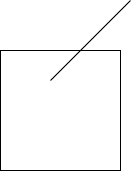
\includegraphics[width=0.3\linewidth]{images/union_example1.png}
        \caption{Voor union.}
        \label{fig:union_example1}
    \end{subfigure}%
    ~ 
    \begin{subfigure}[t]{0.5\linewidth}
        \centering
        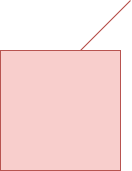
\includegraphics[width=0.3\linewidth]{images/union_example2.png}
        \caption{Resultaat union.}
        \label{fig:union_example2}
    \end{subfigure}
    \caption{Problematiek union.}
\end{figure}

Dit laatste is echter niet mogelijk met de huidige implementatie waar gebruik gemaakt wordt van ``Point'', ``MultiPoint'', ``LineString'', ``MultiLineString'', ``Polygon'' en ``MultiPolygon''. In \figureref{fig:union_example1} is een voorbeeld te zien van twee vormen waarvan de unie (= de vorm die alle punten van beide figuren samen bevat) genomen wordt. In \figureref{fig:union_example2} wordt dan weer aangetoond dat het resultaat van de unie van een ``LineString'' en een ``Polygon'' niet te representeren valt in één van de zes eerder genoemde vormen. Hiervoor zou gewerkt moeten worden met een soort ``GeometryColletion''. 
\newpage
\section{Referentiesysteem}
\label{sec:projecties}
Om een werkende implementatie te bekomen, is er nog een functionaliteit die ondersteund moet worden. Zo moet het mogelijk zijn om te werken met verschillende referentiesystemen. Om nog eens te benadrukken waarom dit belangrijk is, wordt dit geïllustreerd met een voorbeeld. Verschillende landen of zelfs delen van landen liggen op andere aardplaten die los van elkaar bewegen of zelfs tegen elkaar botsen. Hierdoor kunnen landen ten opzichte van elkaar bewegen. Het best voorbeeld hiervan is Australië dat jaarlijks wat kan verplaatsen. Op deze manier zou na enkele jaren elke geografische entiteit opnieuw vastgelegd moeten worden. Hiervoor wordt gebruik gemaakt van aparte referentiesystemen. Dit is een manier om een punt te beschrijven in coördinaten ten opzichte van een relatief punt. Om echter coördinaten in verschillende referentiesystemen te kunnen vergelijken met elkaar, moeten deze eerst omgerekend worden naar hetzelfde referentiesysteem.

Voor het oplossen van dit probleem bestaan twee mogelijkheden. Ofwel worden beide referentiesystemen omgerekend naar één op voorhand gedefinieerd referentiesysteem, ofwel wordt één van beide referentiesystemen naar de andere omgerekend. Er is gekozen voor de tweede optie om twee redenen. In dit geval moet voor elk koppel vormen, dat vergeleken wordt, slechts één vorm herrekend worden, wat zorgt voor een betere performantie. De tweede reden is dat het OGC zelf voorschrijft dat gewerkt moet worden in het referentiesysteem van de eerste vorm.

\subsection{Proj4js}
``Proj4js'' is een \textit{library} die zorgt voor het transformeren van coördinaten van het ene referentiesysteem naar coördinaten van het andere referentiesysteem. Hierbij zijn al enkele projecties op voorhand gedefinieerd binnen Proj4, maar het is ook mogelijk om zelf nieuwe projecties toe te voegen. Proj4 is dan ook de gebruikte \textit{library} voor het uitvoeren van deze berekening bij de gemaakte implementatie.

\subsection{Beperkingen}
Bij deze functionaliteit zijn er nog wel enkele beperkingen. Er zijn nog niet veel referentiesystemen beschreven binnen GeoSPARQL, waardoor het slechts in beperkte mate mogelijk is om van deze functionaliteit gebruik te maken. De architectuur van hoe hiermee gewerkt wordt, is echter wel in orde. Kortom betekent dit dat het nog niet zeer handig is om te gebruiken, maar dat het wel klaar is om in de toekomst toegepast te worden. 
\newpage
\section{Testomgeving}
\label{sec:testomgeving}
\todo{verwijzen hiernaar bij hypothesen}
In de voorgaande secties werd beschreven hoe de implementatie van GeoSPARQL gemaakt is. Nu er een werkende implementatie is, is het mogelijk om over te gaan naar de volgende stap. Hier zijn drie doelen bij, namelijk:
\begin{enumerate}
    \item Visualiseren van het geheel, met makkelijk aanpasbare queries.
    \item Omgeving voor het geven van demonstraties van de implementatie.
    \item Omgeving voor het uitvoeren van tests, voor het aftoetsen van de hypothesen.
\end{enumerate}

Om dit te bereiken is gebruik gemaakt van de ``jQuery Widget'' van Comunica. Deze geeft een grafische \textit{user interface}, die toestaat om te queryen over één of meerdere bronnen. Hierbij is het mogelijk om de bronnen zelf in te geven. Daarnaast is het ook mogelijk om de query zelf in te geven. Deze geeft een overzicht van het resultaat terug en geeft een ``execution log'' terug, zodat gecontroleerd kan worden welke stappen doorlopen werden voor het bekomen van het resultaat. Het geheel hiervan is zichtbaar in \figureref{fig:testomgeving}.

\begin{figure}
    \centering
    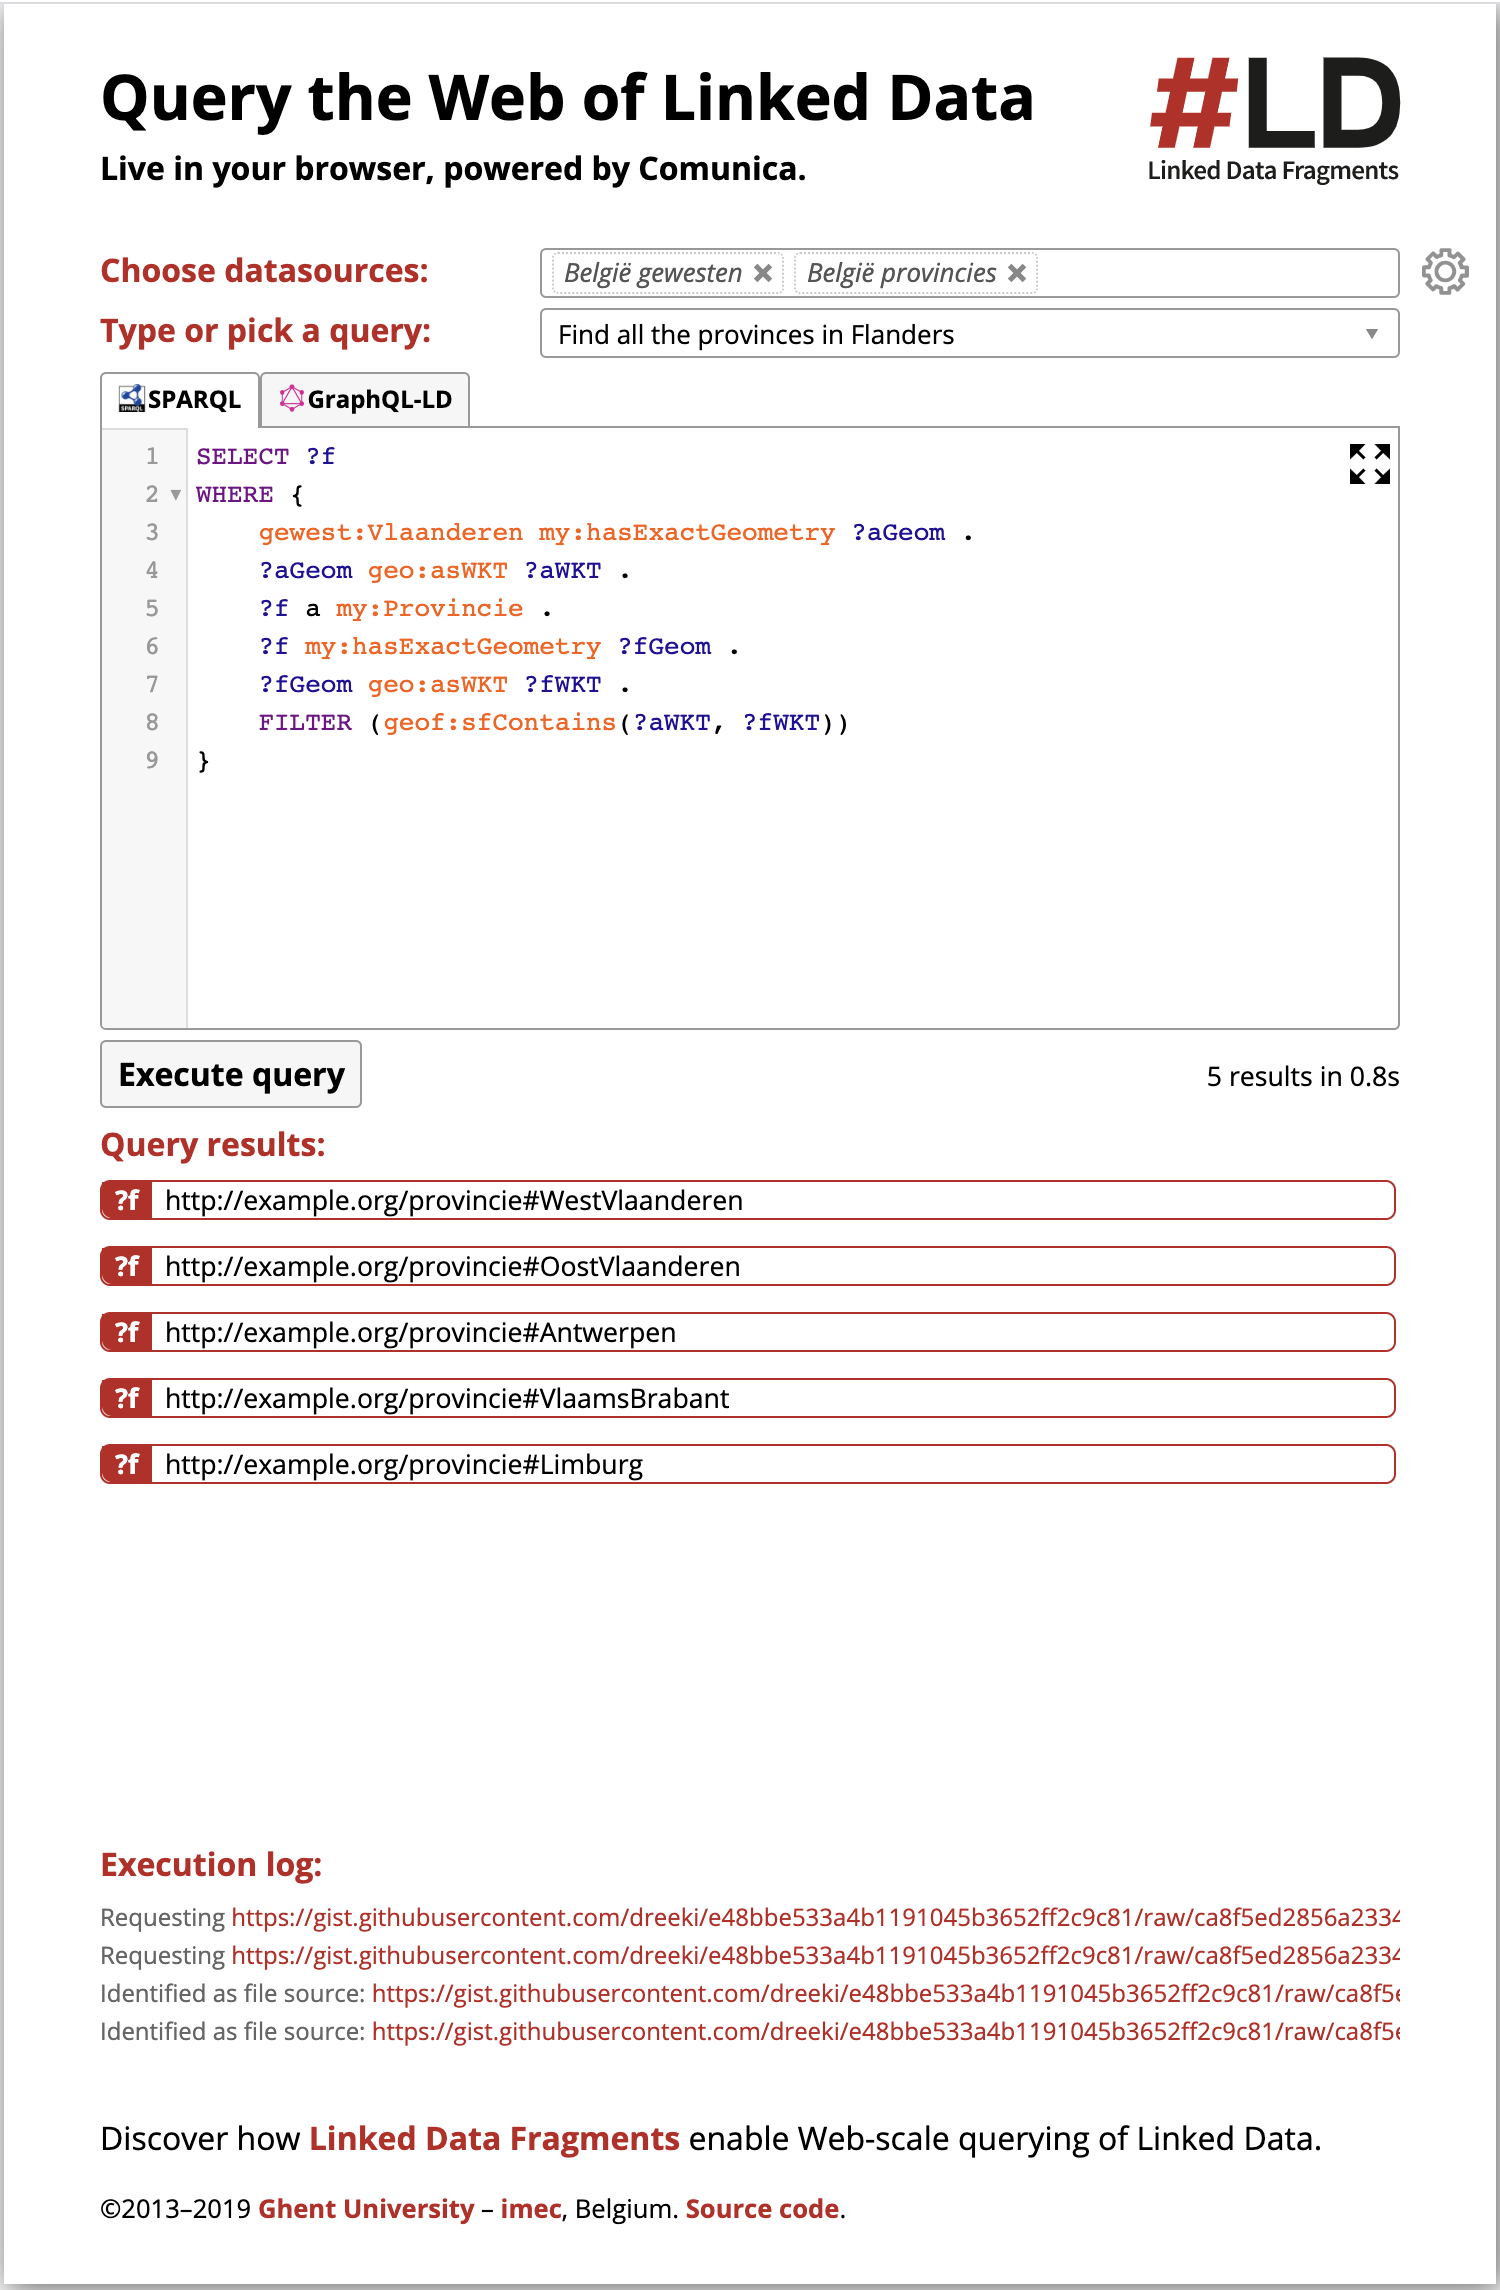
\includegraphics[width=0.8\linewidth]{images/testomgeving.png}
    \caption{Screenshot van online geplaatste testomgeving.}
    \label{fig:testomgeving}
\end{figure}

Hiermee is het eerste doel onmiddelijk bereikt. Dankzij het uitzicht dat zeer gelijkaardig is aan andere gekende \textit{query engines}, is dit zeer geschikt voor het geven van demonstraties. Ten slotte, zoals eerder vermeld, is het mogelijk om zowel de bronnen in te geven als de volgorde van uitvoering te bekijken. Hierdoor is het uitermate geschikt voor het uitvoeren van tests en voor het aftoetsen van de hypothesen. 
\newpage
\section{Overzicht}
\label{sec:impl_overzicht}
Om kort een overzicht te schetsen, zal deze sectie de implementatie overlopen en hierbij beschrijven wat gemaakt is en wat nog te doen is. Bij de vorige secties werden de functionaliteiten besproken in volgorde van implementatie. In dit overzicht zullen ze besproken worden in volgorde van uitwerking. Er kan alleszinds wel besloten worden dat een complete implementatie van GeoSPARQL zeer veel werk vraagt. In het kader van deze masterproef is hier al een deel van gemaakt, maar hier moet nog verder aan gewerkt worden.

\subsection{Huidige status}
Bij deze implementatie wordt eerst gecontroleerd of het gaat over een GeoSPARQL functionaliteit. Wanneer dit het geval is, zal eerst de linker- en rechterparameter recursief opgelost worden, zodat de functionaliteit effectief opgelost kan worden. Bij het oplossen van deze functionaliteit zal eerst de ``WKT string'' omgezet worden naar een GeoJSON object, waarbij gecontroleerd wordt of er een projectie (= referentiestelsel) meegegeven is (indien niet wordt gewerkt met de standaard waarde, genaamd ``WGS84''). Indien beide parameters van de functie niet dezelfde projectie zouden hebben, dan worden de coördinaten van de tweede parameter omgerekend naar de respectievelijke waarden van de projectie van de eerste parameter. Eenmaal dat dit gedaan is kan de functie eenvoudig uitgewerkt worden met behulp van ``Turf.js''. Dit resultaat wordt dan teruggegeven, zodat de boomstructuur dit kan gebruiken voor de verdere uitwerking van de recursieve structuur. Voor niet-topologische functies kan het nodig zijn om een GeoJSON object terug te geven. Om een uniforme werking van sparqlee te kunnen behouden, wordt dit GeoJSON object opnieuw geserialiseerd naar WKT formaat. 

\subsection{Toekomstwerk}
\label{subsec:toekomstwerk}
Aangezien deze implementatie slechts een beperkte implementatie van GeoSPARQL is, zal hier in de toekomst nog verder aan gewerkt moeten worden. Er wordt momenteel slechts in zeer beperkte mate ondersteuning aangeboden voor het gebruik van ``Feature''. Er is ook enkel ondersteuning voor ``WKT strings'' en niet voor het alternatieve ``GML'' formaat. Vervolgens moet er een aanvulling gemaakt worden van zowel de topologische functies als de niet-topologische functies. Bij de topologische functies is enkel gekeken naar de ``Simple Features'' familie (en deze is ook niet helemaal compleet), maar er zijn nog twee andere families. Bij de niet-topologische functies zijn er slechts twee functies geïmplementeerd, zijnde de ``union'' en de ``intersection'' functies. Hier zijn er nog verscheidene andere functies. Ten slotte moet het mogelijk zijn om deze functies te gebruiken in de vorm van predicaat. Hiervoor moet er een functionaliteit zijn voor het herschrijven van de queries. Deze is totaal niet gebruikt, maar is wel nodig voor een volledige implementatie van GeoSPARQL.  
\newpage
\chapter{Interfaces}
\label{chap:interfaces}
Het doel van deze masterproef is het maken van een implementatie van GeoSPARQL in Comunica en te controleren hierbij of het mogelijk is om GeoSPARQL functionaliteiten te implementeren in deze \textit{query engine} die over verschillende heterogene data bronnen kan queryen. Hierbij worden de gegevens op de gebruikelijke manier opgehaald, maar worden de geospatiale relaties uitgerekend op de client-side. Hierbij moet gecontroleerd worden of dit mogelijk is bij de bronnen die momenteel door Comunica ondersteund worden. De belangrijkste bronnen zijn ``data dumps'', ``triple pattern fragment interfaces'' en ``sparql endpoints''. In de komende secties wordt besproken of dit mogelijk is en hoe dit werkt. De eerstvolgende sectie geeft echter een kort overzicht van de gebruikte dataset voor deze tests.

\section{Testset}
\label{sec:testset}
Bij de testset is ervoor gekozen om een oppervlakkige tekening te maken van België in een aangepaste schaal. Deze keuze is gemaakt om meerdere redenen. Om te beginnen laat deze aangepaste schaal zeer gemakkelijk toe om (als mens) vlakken te beschrijven. Aangezien dit een technisch en bovendien vooruitstrevend onderwerp is, is het handig om terug te keren naar een bekender terein. Daarom is de bekendheid van deze \textit{use case} meteen de tweede reden van deze keuze. Een derde reden is dat deze dataset eerder klein is, waardoor mogelijke fouten of onlogische oplossingen hierbij nogmaals getest worden. Ten slotte is dit ook de perfecte dataset voor het geven van demonstraties omdat deze set herkenbaar is voor het publiek. Een visualisatie van deze dataset is te zien in \figureref{fig:demoset}. De effectieve dataset is dan weer te vinden op GitHub Gist\footnote{https://gist.github.com/dreeki/e48bbe533a4b1191045b3652ff2c9c81}. Deze dataset is bovendien opgesplitst in vijf verschillende bestanden (namelijk: ``land'', ``gewest'', ``provincie'', ``weg'' en ``stad'') zodat deze dataset bruikbaar is voor het verifiëren of gefedereerd queryen nog steeds mogelijk is. Het geheel van deze testing wordt uitgevoerd in de testomgeving die besproken werd in \sectionref{sec:testomgeving}. Hierbij zorgt de \textit{execution log} ervoor dat alles duidelijk is hoe het geheel in zijn werk gaat.

\begin{figure}
    \centering
    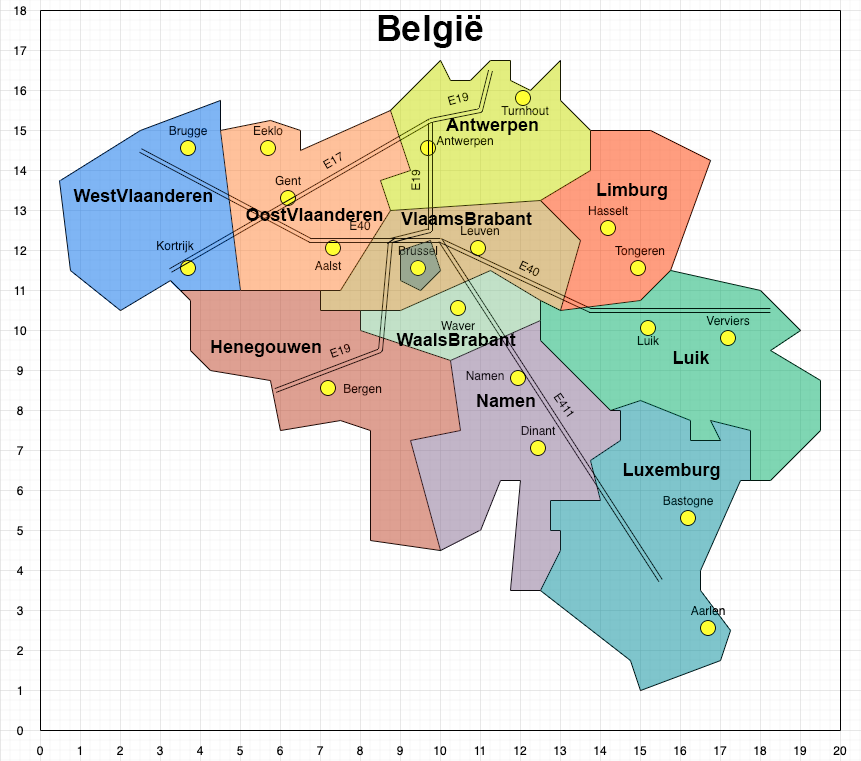
\includegraphics[width=\linewidth]{images/geosparql_demo.png}
    \caption{Testset voor het testen van de verschillende bronnen.}
    \label{fig:demoset}
\end{figure}


\subsection{queries}
Voor de uitvoering van de tests zijn verschillende queries opgesteld om mee te testen. In de testomgeving zelf kunnen hierbij vervolgens de bronnen aangepast worden naar de te testen bronnen. Het is echter wel nog op te merken dat de ontologieën bij de testomgeving reeds in code aangegeven werden. Bij gevolg worden deze niet opnieuw mee opgenomen in de geschreven query, maar in de achtergrond worden deze dus wel nog gebruikt.

\subsubsection{Query 1}
De eerste \textit{query} zoekt naar alle provincies die binnen Vlaanderen liggen. Om dit te kunnen doen zal de \textit{query engine} eerst de vorm van Vlaanderen zelf opzoeken. Daarna zal hij de vorm van alle provincies zoeken zodat hij met de ``sfContains'' functie van GeoSPARQL uiteindelijk kan filteren. Deze query is te zien in \listingref{listing:find_provinces_flanders}.

\begin{listing}[ht]
    \begin{minted}{sparql}
        SELECT ?f
        WHERE {
            gewest:Vlaanderen my:hasExactGeometry ?aGeom .
            ?aGeom geo:asWKT ?aWKT .
            ?f a my:Provincie .
            ?f my:hasExactGeometry ?fGeom .
            ?fGeom geo:asWKT ?fWKT .
            FILTER (geof:sfContains(?aWKT, ?fWKT))
        }
    \end{minted}
    \caption{Find all the provinces in Flanders.}
    \label{listing:find_provinces_flanders}
\end{listing}


\subsubsection{Query 2}
De tweede \textit{query} is zeer gelijkaardig aan de eerste, maar hier is één groot verschil. Deze \textit{query} zoekt naar alles dat binnen Vlaanderen ligt. Aangezien ``sfContains'' functie stelt dat een geospatiaal identieke vorm steeds binnen de andere ligt, zou deze query Vlaanderen zelf ook als een oplossing zien. Aangezien dit niet het verwachte resultaat is, wordt gebruik gemaakt van de negatie van de ``sameterm'' functie van SPARQL. Dit wijst er nogmaals op dat een werkende implementatie van SPARQL een vereiste is voor het maken van een GeoSPARQL implementatie. Deze query is te zien in \listingref{listing:find_everything_flanders}.

\begin{listing}[ht]
    \begin{minted}{sparql}
        SELECT ?f
        WHERE {
            gewest:Vlaanderen my:hasExactGeometry ?aGeom .
            ?aGeom geo:asWKT ?aWKT .
            ?f my:hasExactGeometry ?fGeom .
            ?fGeom geo:asWKT ?fWKT .
            FILTER (geof:sfContains(?aWKT, ?fWKT) && !sameterm(?aWKT, ?fWKT))
        }
    \end{minted}
    \caption{Find everything that's geospatially inside Flanders.}
    \label{listing:find_everything_flanders}
\end{listing}


\subsubsection{Query 3}
De derde query gaat dan weer over het vinden van de wegen en provincies die binnen België liggen. Deze query toont nogmaals aan hoe gelijkaardig SQL en SPARQL zijn. Deze query is te zien in \listingref{listing:find_provinces_roads_belgium}.

\begin{listing}[ht]
    \begin{minted}{sparql}
        SELECT ?f
        WHERE {
            land:België my:hasExactGeometry ?aGeom .
            ?aGeom geo:asWKT ?aWKT .
            {
                ?f a my:Provincie .
            }
                UNION
            {
                ?f a my:Weg .
            }
            ?f my:hasExactGeometry ?fGeom .
            ?fGeom geo:asWKT ?fWKT .
            FILTER (geof:sfContains(?aWKT, ?fWKT))
        }
    \end{minted}
    \caption{Find all the provinces and roads in Belgium.}
    \label{listing:find_provinces_roads_belgium}
\end{listing}


\subsubsection{Query 4}
Bij de vierde query worden alle wegen die door Oost-Vlaanderen gaan opgezocht. Dit zou bijvoorbeeld handig kunnen zijn wanneer iemand de snelwegen wil vinden die eenvoudig bereikbaar zijn vanuit Oost-Vlaanderen. Hierbij wordt de functie ``sfIntersects'' van GeoSPARQL gebruikt. Deze query is te zien in \listingref{listing:find_roads_passing_east_flanders}.

\begin{listing}[ht]
    \begin{minted}{sparql}
        SELECT ?f
        WHERE {
            prov:OostVlaanderen my:hasExactGeometry ?aGeom .
            ?aGeom geo:asWKT ?aWKT .
            ?f a my:Weg .
            ?f my:hasExactGeometry ?fGeom .
            ?fGeom geo:asWKT ?fWKT .
            FILTER (geof:sfIntersects(?aWKT, ?fWKT))
        }
    \end{minted}
    \caption{Find all the roads that pass through East-Flanders.}
    \label{listing:find_roads_passing_east_flanders}
\end{listing}


\subsubsection{Query 5}
De vijfde query toont aan dat het mogelijk is om manueel een vorm te voorzien om op te filteren. Deze vorm staat (bij de aangepaste schaal) voor de \textit{bounding box} van Vlaams-Brabant en Waals-Brabant. Deze query zal alles weergeven dat zich binnen deze vorm bevindt. Voor de verandering wordt hier de ``sfWithin'' functie van GeoSPARQL gebruikt, maar dit zou evengoed mogelijk zijn met de ``sfContains'' functie. Deze query is te zien in \listingref{listing:find_everything_bounding_box}.

\begin{listing}[ht]
    \begin{minted}{sparql}
        SELECT ?f
        WHERE {
            ?f my:hasExactGeometry ?fGeom .
            ?fGeom geo:asWKT ?fWKT .
            FILTER (geof:sfWithin(?fWKT, '''Polygon((7 9.25, 13.5 9.25, 13.5 13.25, 
            7 13.25, 7 9.25))'''^^geo:wktLiteral))
        }
    \end{minted}
    \caption{Find everything inside the bounding box of Brabant.}
    \label{listing:find_everything_bounding_box}
\end{listing}




\todo{misschien nog extra queries} 
\newpage
\section{Data dump}
\label{sec:data-dump}
De eerste bron om te controleren, wordt gebruikt als baseline. Dit is de ``data dump''. Dit is een gewoon bestand in RDF formaat dat door de \textit{query engine} opgehaald (lees gedownload) wordt. Vervolgens wordt het door de \textit{query engine} gecontroleerd of het effectief wel een bestandsbron is. Eenmaal dit voldaan is, worden steeds de kleinste patronen gezocht die voldoen aan de bron. Dit is nodig omdat de \textit{query engine} zo op de meest performante manier de \textit{joins} kan uitvoeren. Zo kan ten slotte de filter-functie de overbodige oplossingen weghalen. Deze filter-functie is voorzien door GeoSPARQL. Bovendien voorziet Comunica functionaliteiten om data-entiteiten uit de databron te extraheren, wat hier gebeurt op de client. Over deze entiteiten moet een filter functie geëvalueerd kunnen worden. Hierdoor is het mogelijk om data dumps te queryen met GeoSPARQL. Aangezien data dumps letterlijk bestanden zijn zonder een eigen voorziening van logica, is het triviaal dat dit afgehandeld moet kunnen worden. De data dump wordt daarom de \textit{baseline} van dit onderzoek, waarbij er gepoogd wordt om dezelfde resultaten bij andere bronnen ook te behalen.

Bij het testen van de data dump worden de GitHub Gist bestanden (zie \sectionref{sec:testset}) rechtstreeks gebruikt. Hier is geen enkel ander programma dat als aanspreekpunt gebruikt wordt. Hierbij is dus ook duidelijk dat het beschreven proces van hierboven correct doorlopen is. Dit is bovendien de manier van werken die gebruikt is bij het maken en testen van de implementatie. 
\newpage
\section{Triple pattern fragment interface}
\label{sec:impl_tpf_interface}
De volgende bron is de ``triple pattern fragment interface''. Dit is een server die tussen de op te vragen bestanden (dus de effectieve gegevens) en de client staat. Deze server zal ervoor zorgen dat het niet langer nodig is om alle data op te halen, maar in de plaats zal de server de SPARQL query splitsen in verschillende triple pattern fragment requests. Deze vragen alle triples die voldoen aan een enkel tripple pattern fragment en \textit{joinen} dan de resultaten op de client. De filtering gebeurt daarna ook op de client.

Net zoals bij de data dump (zie \sectionref{sec:data-dump}) vraagt de \textit{query engine} de bron op. Hierbij zal hij de bron identificeren als een ``qpf source'', wat staat voor ``Quad pattern fragment''. Dit is eigenlijk de \textit{triple pattern fragment} met hierbij een extra veld (graph) toegevoegd, maar hier wordt niet verder op in gegaan. Vervolgens begint de \textit{query engine} de query op de splitsen in TPF queries, zodat deze TPF queries geoptimaliseerd kunnen worden in een volgorde die gebaseerd is op de initiële count query. Hierna worden deze één voor één uitgevoerd. Zo zal hij vervolgens de kleinste patronen opvragen, zodat de correcte informatie opgevraagd kan worden met hierbij een minimale hoeveelheid aan overbodige informatie mee te krijgen. Dit is enkel mogelijk dankzij de TPF interface. Dankzij deze manier van werken kan wederom de uiteindelijke filtering van de \textit{queries} louter op de client-side gebeuren.

Voor het opzetten van deze test is gebruik gemaakt van de ``Linked Data Fragments Server''. Deze bouwt een TPF interface op boven een set van bronbestanden, waarvoor opnieuw de bestanden van GitHub Gist gebruikt zijn, net zoals bij de data dump. Op deze manier is ook verzekerd dat er met dezelfde gegevens gewerkt wordt. 

Als kleine opmerking kan nog vermeld worden dat een TPF interface gebruikt wordt voor twee redenen. Ten eerste hoeft de client zo niet alle data te downloaden, maar kan de server slechts een fragment (vandaar de naam, deze komt eigenlijk van ``Linked Data Fragments'') van deze data teruggeven. De tweede reden is dat deze filtering meestal (= niet in alle gevallen) zorgt voor een verbeterde performantie. Bij het testen was dit echter niet terug te vinden. Zo blijkt het uitvoeren van de queries met de data dump sneller te gaan dan met de TPF interface. Hier is echter een logische verklaring voor. De datasets dit gebruikt zijn, zijn relatief gezien kleine datasets. Bovendien bevatten deze enkel de noodzakelijke gegevens, waardoor de dataset volledig nodig is voor het uitvoeren van de query. Hierdoor kan er niet genoten worden van de voordelen van de TPF interface, maar wordt enkel de extra \textit{overhead} waargenomen. Dit gaat echter buiten de \textit{scope} van deze scriptie, daarom werd hier verder geen onderzoek naar gedaan, noch benchmarking van de performantie. Dit is eerder een opmerking bij de ondervindingen. 
\newpage
\section{SPARQL endpoint}
\label{sec:impl_sparql_endpoint}
De laatste bron om te testen is meteen de moeilijkste. Bij het SPARQL endpoint is het de bedoeling dat een GeoSPARQL query uitgevoerd kan worden door de gegevens op te vragen aan dit SPARQL endpoint. Comunica zelf is gemaakt om queries uit te voeren over RDF bronnen, wat het zeer handig maakt om SPARQL queries uit te voeren. Hierdoor lijkt het logisch om de query in zijn geheel door te sturen in het geval van een SPARQL endpoint als bron. Dit SPARQL endpoint is namelijk in staat om volledig automoon een antwoord te geven op de query. Dit is echter niet hoe het in zijn werk gaat. Eén van de redenen hiervoor is dat gefedereerd queryen zo niet mogelijk zou zijn wanneer er naast het SPARQL endpoint nog een andere bron zou zijn. Zo moet de samenvoegingen van de antwoorden op de client-side gebeuren. 

Bij een SPARQL endpoint zal de \textit{query engine} de verschillende RDF triples van de query overlopen. Dit doet hij in twee stappen. De eerste stap is een ``count'' zodat hij weet hoeveel RDF triples van de bron overeen komen met de RDF triples van de query. Dit wordt gedaan zodat de \textit{query engine} weet welke volgorde optimaal is om de data op te halen, zodat hij dit optimaal kan joinen. De tweede stap is het effectieve ophalen van het resultaat, waarbij hij dus alle antwoorden vraagt die voldoen aan slechts één RDF triple van de query. Wanneer dit voor alles gedaan is zoekt hij het kleinste patroon, zodat hij vervolgens de matchende RDF triples kan ophalen. Het kleinste patroon wordt gekozen om het aantal matchende resultaten te minimaliseren voor performantie redenen.

Zo wordt uiteindelijk alle benodigde informatie uit het SPARQL endpoint systematisch opgehaald, zodat de filter bij de oorspronkelijke query onafhankelijk van de bronnen kan uitgevoerd worden. Dit betekent ook dat de filter functies steeds dezelfde implementatie hebben (namelijk deze van de \textit{query engine} op de client, niet deze van de bron). Dit laat echter ook toe om te filteren met de GeoSPARQL functies. Dankzij deze werkwijze is het dus effectief mogelijk om de GeoSPARQL functionaliteit toe te passen bij het opvragen aan een SPARQL endpoint. 
\newpage
\begin{savequote}[0.55\linewidth]
	``Dream big and dare to fail.''
	\qauthor{\textasciitilde 
    Norman Vaughan}
\end{savequote}

\chapter{Conclusie}
\label{chap:conclusie}
In dit hoofdstuk worden de resultaten, besproken in \chapterref{chap:interfaces}, geïnterpreteerd. Er wordt een antwoord geformuleerd op de vragen uit \sectionref{sec:onderzoeksvraag}.

\textbf{Onderzoeksvraag: Welke ``Linked Data publicatie''-interfaces kunnen uitgebreid worden met GeoSPARQL-functionaliteiten door de filtering op de client uit te voeren?}

De masterproef brengt een oplossing om de ``Linked Data publicatie''-interfaces uit te breiden met GeoSPARQL-functionaliteiten. Dit betekent dat er gelinkte data online gepubliceerd worden. Deze data kunnen opgehaald worden met behulp van SPARQL (zie \sectionref{sec:sparql}). 

De vraag is hoe deze opvraging kan uitgebreid worden met GeoSPARQL-functionaliteiten. Hiervoor wordt gebruik gemaakt van de al bestaande implementatie van Comunica. Door Comunica uit te breiden met deze GeoSPARQL-functionaliteiten wordt gepoogd om op dezelfde manier te kunnen werken als voordien, maar ditmaal met GeoSPARQL-functionaliteiten. Specifiek hierbij worden de data opgehaald en gefilterd op de client zelf (zoals besproken in \chapterref{chap:interfaces}).

De meest voorkomende ``Linked Data publicatie''-interfaces voor het gebruik van geospatiale data zijn ``data dumps'', ``\acrshort{tpf} interfaces'' en ``SPARQL endpoints''.

\textbf{Hypothese 1: Het is mogelijk om GeoSPARQL queries uit te voeren over ``data dumps'' waarbij de filtering op de client-side gebeurt.}

Bij een ``data dump'' worden de data volledig gedownload op de client. Hier zal de client vervolgens de resultaten joinen zoals nodig in de query. Ten slotte zal de client over de volledige dataset filteren, om zo tot het correcte resultaat te komen. 

Hieruit volgt dat Hypothese 1 correct is.

\textbf{Hypothese 2: Het is mogelijk om GeoSPARQL queries uit te voeren over ``\acrshort{tpf} interfaces'' door de filtering op de client-side uit te voeren.}

De ``\acrshort{tpf} interface'' is een server die een dataset bevat. Deze server bevat functionaliteiten om te kunnen antwoorden op vragen naar een \textit{triple pattern fragment}. Zo wordt de volledige query opgesplitst, zodat de ``\acrshort{tpf} interface'' het kleinst mogelijke deel van de dataset (dat alle vereiste data bevat) kan terug geven. Hierbij zal de client wederom de resultaten joinen om hierop te kunnen filteren zodat het correcte resultaat bekomen kan worden.

Hieruit volgt dat ook Hypothese 2 correct is.

\textbf{Hypothese 3: Het uitvoeren van GeoSPARQL queries op een ``SPARQL endpoint'' is niet vanzelfsprekend. Het is echter mogelijk door de filtering op de client-side uit te voeren.}

Een ``SPARQL endpoint'' is zelfstandig in staat om te antwoorden op een SPARQL query. Hierbij is er geen optie om een GeoSPARQL query door te sturen omdat het ``SPARQL endpoint'' hier niet kan op antwoorden. Bij een ``SPARQL endpoint'' wordt dit probleem aangepakt door niet de volledige query door te sturen, maar in de plaats te tellen hoeveel antwoorden er zijn op elk \textit{triple pattern fragment} in de query. Zo kan de client zelf beslissen welk fragment nodig is om het kleinst mogelijke patroon te vinden. Hierdoor kan het joinen van het resultaat op de client gebeuren. Ook hierbij is dus de laatste stap om het resultaat te filteren op de client. 

Hieruit volgt dat ook Hypothese 3 correct is.

\section{Toekomstig werk}

De gemaakte implementatie is slechts een beperkte implementatie van GeoSPARQL (zoals vermeld in \subsectionref{subsec:toekomstwerk}). Bij verdere implementatie hiervan moet gecontroleerd worden in hoeverre de libraries (zoals ``Turf'' en ``Proj4'') de vereiste functionaliteiten correct ondersteunen. Enerzijds voorziet Turf een groot arsenaal aan geospatiale functionaliteiten, maar wanneer deze niet helemaal kloppen met de verwachtingen is het niet mogelijk om deze manueel aan te passen, om andere conclusies te trekken. Hierbij zou het een meerwaarde zijn om een \textit{library} te maken die eerder werkt op basis van de DE-9IM intersectie. Hiermee wordt bedoeld dat de DE-9IM intersectie aangegeven zou worden door deze nieuwe \textit{library}. Aan de hand van DE-9IM worden alle vereisten van de GeoSPARQL-functionaliteiten uitgedrukt. Zo zou het eenvoudiger zijn om een specifieke functionaliteit van GeoSPARQL correct te implementeren. 

Verder zou het ideaal zijn, moest Sparqlee uitgebreid worden met \textit{custom} functies, zodat de GeoSPARQL-functionaliteiten in Comunica zelf geïmplementeerd kunnen worden. Deze zouden dan geïnjecteerd moeten worden in Sparqlee. Op deze manier kan de modulariteit van Comunica volledig benut worden.

Als laatste blijft het steeds een zoektocht naar de meest performante manier om alle data te verwerken. In deze masterproef werd rekening gehouden met performantie, maar aangezien dit niet de focus was, is hier niet te diep op ingegaan. Zo dient er een benchmarking te gebeuren ter controle of de gemaakte oplossingen schaalbaar zijn.

\section{Tot slot}
In deze masterproef is een implementatie gemaakt van GeoSPARQL. Zoals besproken in \chapterref{chap:implementatie} is deze implementatie grotendeels gemaakt in Sparqlee, met een eigen GeoSPARQL actor in Comunica. Hierbij is gebruik gemaakt van de libraries ``Turf'', ``Proj4'' en ``Terraformer''. Bij deze implementatie is bovendien een client gemaakt, zodat dit geheel in een visuele omgeving zichtbaar is. Deze omgeving voorziet voldoende logs om te controleren hoe alles samenwerkt. Daarnaast is het mogelijk om de performantie te controleren, aangezien deze client meegeeft hoelang de query duurde om uit te voeren. 

Vervolgens werd deze implementatie toegepast in \chapterref{chap:interfaces}. Hierbij werd getest of de verschillende interfaces uitgebreid konden worden met GeoSPARQL-functionaliteiten. In dit hoofdstuk wordt beschreven hoe het geheel in zijn werk gaat. Aan de hand van deze beschrijving wordt nogmaals duidelijk waarom het filteren op de client belangrijk is. 

In \chapterref{chap:conclusie} worden deze resultaten opnieuw geïnterpreteerd. Zo kan een concreet antwoord gevormd worden op de hypotheses die gesteld zijn in \sectionref{sec:onderzoeksvraag}. Tot slot kan geconcludeerd worden dat deze hypotheses correct zijn. Dit betekent dat zowel ``data dumps'', als ``\acrshort{tpf} interfaces'', als ``SPARQL endpoints'' uitgebreid kunnen worden met GeoSPARQL-functionaliteiten door de filtering op de client uit te voeren.
\bibliography{data/references.bib}


\todo{images/ weghalen}
\todo{citaat bij begin van een hoofdstuk is fancy}
\todo{zoeken naar data en informatie, mogelijks vervangen door gegevens}
\todo{acroniemen en moeilijke woorden tonen! (TPF, W3C)}
\todo{captions naar nederlands}
\todo{query altijd schuin!}
\todo{vervangen scriptie en thesis door masterproef}
\todo{bij elk blad staat de nummering met een puntje teveel}

\end{document}